\documentclass[11pt]{amsart}

\usepackage[dvipsnames]{xcolor}
\usepackage{amssymb,mathtools}
\usepackage[letterpaper,margin=1in]{geometry}
\usepackage[citecolor=PineGreen,colorlinks=true,linkcolor=RoyalBlue,urlcolor=BrickRed]{hyperref}
\usepackage{graphicx}
\usepackage{tikz}
\usetikzlibrary{arrows.meta,decorations.pathreplacing}

\theoremstyle{plain}
\newtheorem{theorem}{Theorem}[section]
\newtheorem{proposition}[theorem]{Proposition}
\newtheorem{definition}[theorem]{Definition}
\newtheorem{lemma}[theorem]{Lemma}
\newtheorem{corollary}[theorem]{Corollary}
\theoremstyle{definition}
\newtheorem*{assumptionU}{Assumption \textup{(U)}}
\theoremstyle{remark}
\newtheorem{remark}[theorem]{Remark}


\newcommand{\E}{\mathbb{E}}
\newcommand{\Zd}{\mathbb{Z}^d}
\newcommand{\Rd}{\mathbb{R}^d}
\newcommand{\R}{\mathbb{R}}
\newcommand{\Z}{\mathbb{Z}}
\renewcommand{\a}{\mathbf{a}}
\newcommand{\cu}{\square}
\renewcommand{\O}{\mathcal{O}}
\newcommand{\eps}{\varepsilon}
\renewcommand{\P}{\mathbb{P}}
\newcommand{\Var}{\text{Var}}


\title[Homogenization for the critical long-range random conductance model]{Quantitative homogenization for the critical long-range random conductance model}


\author{Ahmed Bou-Rabee}
\address{Department of Mathematics, University of Pennsylvania, Philadelphia, PA 19104}
\email{ahmedmb@sas.upenn.edu}

\author{Paul Dario}
\address{Laboratoire AGM, CY Cergy Paris Universit\'e, 95302 Cergy-Pontoise, France}
\email{paul.dario@cyu.fr}

\begin{document}
	
	\begin{abstract}
		We consider the long-range random conductance model on $\mathbb{Z}^d$ at the critical exponent: the jump rate between sites $x$ and $y$ decays as $\a(x,y) |x-y|^{-(d+2)}$, where~$\a(x,y)$ are i.i.d.\ uniformly elliptic conductances.
		Below the critical exponent~$(d+2)$ the walk converges to a stable process; above it, to Brownian motion with diffusive $\sqrt{t}$ scaling.
		At criticality the second moment of the jump kernel diverges logarithmically.
		We establish quantitative homogenization of the associated elliptic equation to the Laplacian at the rate $1/\sqrt{|\ln\varepsilon|}$.
		As a consequence, we deduce quenched convergence of the random walk to Brownian motion under the anomalous~$\sqrt{t \log t}$ scaling.
		Unlike in standard homogenization, the effective diffusivity is determined by the mean conductance alone, with no corrector contribution at leading order.
	\end{abstract}
	
	
	
	
	\maketitle

% ---------------------------------------------------------------------------
% REVISED DRAFT. This file is a locally corrected copy of arXiv:2604.21143v1
% (original source critical-long-range-rw.tex, SHA-256 1fec0f85...a627, unchanged).
% The abstract is unchanged. Each change is marked "% REVISED" in the source.
% ---------------------------------------------------------------------------
\section*{Corrections relative to arXiv:2604.21143v1}
\begin{enumerate}
\item[(C1)] Introduction, after (1.2): ``$\kappa_\eps \asymp |\ln\eps|$'' is replaced by
``$\kappa_\eps \asymp 1+|\ln\eps|$''. For $\eps\in(\tfrac12,1)$ the $2d$ unit vectors give
$\kappa_\eps\ge 2d$ while $|\ln\eps|\to0$; every later use only needs the corrected
comparison (as already stated in Appendix~B). Formal counterparts: \texttt{LongRange.kappa\_le},
\texttt{LongRange.le\_kappa}.
\item[(C2)] Proof of Proposition~\ref{p.dirichlet}, Step~3: ``$|U^\eps|\asymp\eps^{-d}$'' is
replaced by ``$|U^\eps|\le C\eps^{-d}$''. Only the upper bound is used; the lower bound fails when
$\eps$ is large compared with $U$ (then $U^\eps$ may be empty). Formal counterpart:
\texttt{LongRange.ncard\_latticeSet\_le}.
\item[(C3)] Proof of Proposition~\ref{p.dirichlet}, display~\eqref{eq:upperboundsigmaSR}: the
factor $|\ln\eps|$ is replaced by $1+|\ln\eps|$. As $\eps\uparrow1$ only nearest-neighbour
increments satisfy $\eps\le|v|<1$, so $\Sigma_p^{\mathrm{SR}}(x+z,x)$ reduces to
$(\E[\a]-\a(x,x+z))J(z)(p\cdot z)$, which does not vanish, while $|\ln\eps|\to0$. The influence
bound that follows is unchanged because $(1+|\ln\eps|)/\kappa_\eps\le C$. Formal counterpart:
\texttt{LongRange.shortCoeff\_abs\_sum\_bound} (internal to the proof of Proposition~\ref{p.dirichlet}).
\end{enumerate}
\noindent\emph{Confirmed gap in a proof (statement believed true).} (G1) The proof of
Proposition~\ref{p.heatkernel.offdiag} applies \cite[Theorem~1.12]{ChenKumagaiWang2019} on
$\Zd$ with counting measure; its all-radius hypotheses (FK and, through
\cite[Proposition~2.1]{ChenKumagaiWang2019}, RVD) fail at radii below one, so the printed proof
is invalid. Section~6 uses the proposition only through the displacement bound
\eqref{e.displacement.tail}, for a fixed realization, with constants that may depend on it.
Proposed repair of the proof only (statement and Section~6 unchanged; verified against
arXiv:2010.05414v1, journal text not compared): Meyer truncation of the jumps at
$\rho=\gamma|x-y|$, the comparison $p^\rho_t\le e^{C_\rho t}p_t$, the Davies-type bound of
Chen--Kim--Kumagai--Wang (J.~Funct.\ Anal.\ 281 (2021) 109074), Theorem~4.4 with Example~4.3,
fed by the Nash inequality of their Proposition~3.1(ii) and the on-diagonal profile
$[t(1+\log(1+t))]^{-d/2}$ of Proposition~\ref{p.heatkernel}, a tent test function, and the
Duhamel/Meyer comparison. The repair is written out in Appendix~\ref{sec:heatkernel} (proof of
Proposition~\ref{p.heatkernel.offdiag}). Formal counterpart: \texttt{LongRange.Statements.heatkernel\_offDiagonal}
(provider \texttt{LongRange.unitHeat\_offDiagonal\_uniform}), with the cited results of
\cite{MuruganSaloffCoste2015} and Chen--Kim--Kumagai--Wang as explicit hypotheses.

\noindent\emph{Constant dependence clarified; statements unchanged.} (O2)
Propositions~\ref{p.heatkernel} and~\ref{p.heatkernel.offdiag} retain the original
constant $C=C(d,\lambda)$, uniformly over all admissible conductances.
In the proof of \cite[Theorem~1.1]{MuruganSaloffCoste2015}, the kernel dependence
is through its jump-comparison constant. The fixed lattice, volume and scale
profiles and a common jump-comparison constant therefore give one heat-kernel
constant for every admissible conductance field. The proof below uses a common
uniformization rate and states this dependence explicitly. No weaker
configuration-dependent formulation is substituted for either proposition.

\noindent\emph{Audit concern (not a confirmed error).} (O3) Proof of
Proposition~\ref{p.corrector.domain}: ``for $\eps > 1/2$ the bound holds trivially since $U^\eps$ has
$O(1)$ points'' is not an argument (the energy sums over all edges touching $U^\eps$, and the affine
part has a logarithmically divergent second moment). The bound is true: the proof of
Proposition~\ref{p.dirichlet} gives, for every $\eps \in (0,1)$, the estimate with $|\ln\eps|$ replaced
by $\kappa_\eps$, from which both propositions follow using $\kappa_\eps \ge c(1+|\ln\eps|)$.

\noindent\emph{Audit concern (not a confirmed error).} (O4) Proof of Theorem~\ref{main.thm}, Step~5:
Proposition~\ref{p.corrector.domain} is applied to the cubes $V_m^{\widehat\eps_m}$ with a constant
claimed uniform in $m$ because their diameters are bounded; the proposition as stated has
$C = C(d,\lambda,U)$ for one $U$. Choosing $\widehat\eps_m = w_U 3^{-m}$ ($w_U$ the side of the smallest
cube containing a translate of $U$) makes $V_m^{\widehat\eps_m}$ one fixed cube, so the stated
proposition suffices.

\noindent\emph{Citation refinement.} (R1) Proof of Theorem~\ref{main.thm}, first paragraph: the
constants ``depending only on $\mu, d, \lambda, \sigma, U$ and $\|f\|_{C^{0,\sigma}}$'' follow from
\cite{GilbargTrudinger2001}, Theorems~6.19 (regularity), 6.6 (Schauder estimate) and 3.7 (maximum
principle), and the extension $\widetilde u_\mu$ from Lemma~6.37 of the same book (in place of the
uncited Stein extension theorem); these results are stated for $d \ge 2$. In dimension $d = 1$ the
corresponding facts are elementary (ODE on an interval) and are proved directly.

\noindent\emph{Stopping-time convention and citation clarified.} (O5)
The finite-horizon Aldous criterion uses stopping times for the natural
filtration of the corresponding process. Its vector-valued, finite-horizon form
follows from the stopping-time compactness criterion in
\cite[Chapter~3, Theorem~8.6(c) and Remark~8.7(b)]{EthierKurtz1986}, together with
finite-horizon Skorokhod complete metrizability
\cite[Theorems~12.1 and 12.2]{Billingsley1999}. The adapters retain the terminal
value and the full sequence of laws. This specifies the intended filtration
without changing the criterion's two conditions. Initial laws, including time
zero, are included in the finite-dimensional convergence argument.

\noindent\emph{Simplified route (adopted).} (A1) Section~\ref{sec:convergence} can be argued
without the Euler approximation and without the boundary continuity of (O6). For a ball $B_R$, the
killed generators act on $L^2(B_R)$ and $\ell^2(B_R \cap \eps\Zd)$, compared through cell averages.
Theorem~\ref{main.thm}, applied to smooth compactly supported data on a countable dense set, gives
convergence of the killed resolvents on one full-probability event for all $L^2(B_R)$ data and all
integers $R \ge 1$. The Trotter--Kato theorem for varying spaces~\cite[Theorem~1.6.1]{EthierKurtz1986}
then gives uniform convergence of the killed semigroups on bounded time intervals, and a backward
recursion through bounded multipliers gives convergence of the killed finite-dimensional expectations
against the killed Brownian motion; the killing is removed as $R \to \infty$ since the exit probability of
a ball before a fixed time vanishes. Together with relative compactness
of the laws on $D([0,\infty);\Rd)$ (from the displacement estimate~\eqref{e.displacement.tail} and
\cite[Chapter~3, Theorem~8.6]{EthierKurtz1986}), this identifies the limit by
\cite[Chapter~3, Theorem~7.8]{EthierKurtz1986}. Proposition~\ref{p.tightness} likewise follows from this
relative compactness: the expected increments across the time $T$ are uniformly small by the
displacement estimate, so no limit law has a fixed jump at $T$; restriction to $[0,T]$ is continuous at
paths without a jump at $T$, so the restricted laws are relatively compact, hence tight because $D([0,T];\Rd)$
is Polish~\cite[Theorems~12.1 and 12.2]{Billingsley1999}.

\noindent\emph{Audit concern (not a confirmed error).} (O6) Proof of Theorem~\ref{t.qip}: the
continuity up to the boundary of $P^U_t h$ for $h \in C(\overline U)$ and $t > 0$ (killed Brownian
motion on a ball) is attributed to the Feller property in \cite[Section~4.2]{EthierKurtz1986}; that
section concerns semigroups on $C_0$ and does not by itself give this boundary regularity, which holds
for balls by the regularity of their boundary points.
% ---------------------------------------------------------------------------

	
	\section{Introduction}
	
	\subsection{The critical long-range random conductance model}
	
	Consider a random walk on $\Zd$ whose jump rate from $x$ to $y$ is
	\begin{equation}
		\label{e.jump.rates}
		c(x,y) = \a(x,y) \cdot |x - y|^{-(d+\alpha)}\,,
	\end{equation}
	where $\alpha > 0$ and the conductances $\{\a(x,y)\}$, indexed by unordered edges $\{x,y\}$, are i.i.d.\ and satisfy $\lambda \le \a(x,y) \le \lambda^{-1}$ almost surely for a fixed $\lambda \in (0,1]$.
	The exponent $\alpha$ controls the large-scale behavior.
	For $\alpha < 2$, the rescaled walk converges to an $\alpha$-stable process~\cite{ChenKumagaiWang2021,ChenChenKumagaiWang2025}.
	For $\alpha > 2$, it converges to Brownian motion~\cite{BiskupChenKumagaiWang2021}.
	At the critical value $\alpha = 2$, the second moment $\sum_{z \in \Zd \setminus \{0\}} |z|^{-d}$ diverges logarithmically.
	This paper considers the critical case: we prove quantitative homogenization of the associated elliptic equation at the rate $1/\sqrt{|\ln\eps|}$ and deduce a quenched invariance principle.
	The effective diffusivity of the homogenized elliptic equation is $\E[\a(0,e_1)]/(2d)$, with no corrector contribution at leading order.
	
	\begin{figure}[ht]
		\centering
		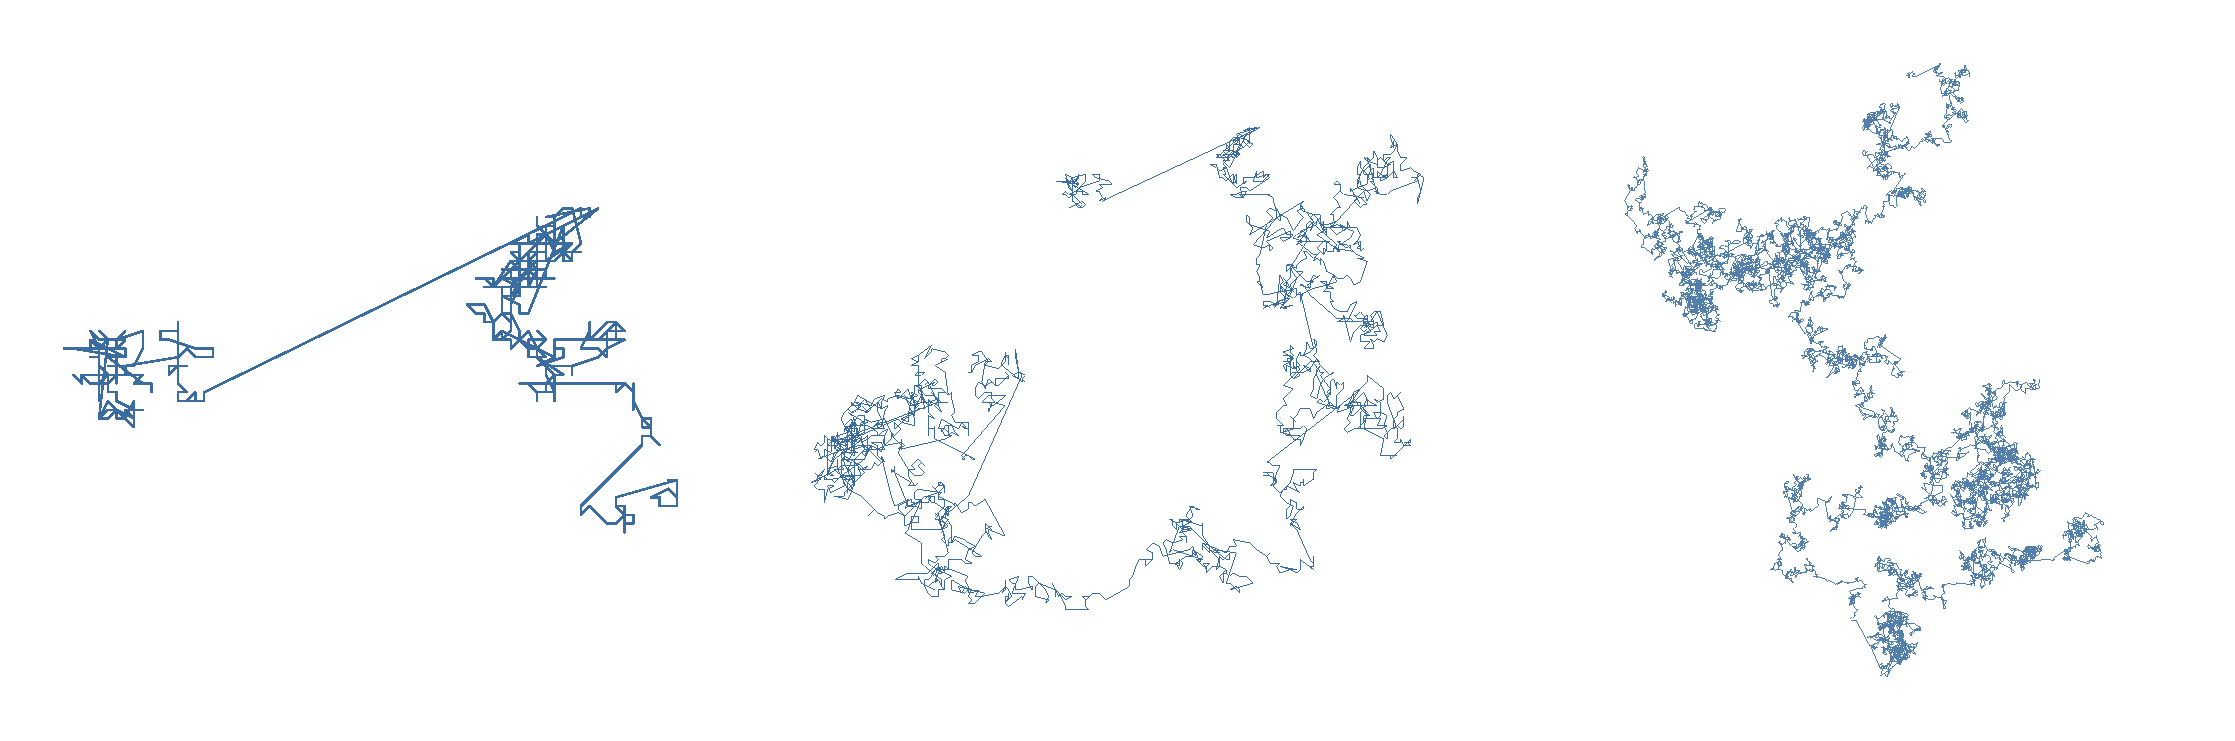
\includegraphics[width=\textwidth]{critical_rw_convergence.pdf}
		\caption{A sample path of the critical long-range random walk on $\Z^2$ with jump kernel $|z|^{-4}$ and random conductances, shown at three successive scales: $500$ steps (left), $5{,}000$ steps (center), and $100{,}000$ steps (right). By Theorem~\ref{t.walk.intro}, the walk converges to Brownian motion under $\sqrt{t \log t}$ scaling.}
		\label{fig:qip}
	\end{figure}
	
	\subsection{Main results}
	
	For a lattice spacing $\eps > 0$ and a function $h \colon \eps\Zd \to \R$, define the rescaled nonlocal operator
	\begin{equation}
		\label{e.Leps}
		\mathcal{L}^\eps h(x) \coloneqq \frac{\eps^d}{\kappa_\eps}
		\sum_{z \in \eps\Zd \setminus \{0\}}
		\a\left(\frac{x}{\eps}, \frac{x+z}{\eps}\right)
		\frac{h(x+z) - h(x)}{|z|^{d+2}}\,,
	\end{equation}
	where $\kappa_\eps \asymp 1 + \left| \ln\eps \right|$ normalizes the logarithmically divergent second moment (see~\eqref{e.kappaeps} for the precise definition). % REVISED: see correction list
	
	\begin{assumptionU}\label{a.U}
		Let $d \ge 1$ be an integer, let $\lambda \in (0,1]$, and let $\a = \{\a(x,y)\}_{x \ne y}$ be i.i.d.\ symmetric random conductances indexed by unordered edges, satisfying $\a(x,y) = \a(y,x)$ and $\lambda \le \a(x,y) \le \lambda^{-1}$.
	\end{assumptionU}
	
	\begin{theorem}[Quantitative homogenization]
		\label{main.thm}
		Under Assumption~\textup{(U)}, let $\sigma \in (0,1)$, let $\mu \ge 0$, let $U \subset \Rd$ be a bounded domain with $C^{2,\sigma}$ boundary, and let $f \in C^{0,\sigma}(\bar U)$.
		For $\eps \in (0,1)$, let $u^\eps_\mu \colon \eps\Zd \to \R$ and $\bar u_\mu \in H^1_0(U)$ be the solutions of
		\begin{equation}
			\label{e.main.equations}
			\left\{
			\begin{aligned}
				\mu u^\eps_\mu - \mathcal{L}^\eps u^\eps_\mu &= f && \text{in } U \cap \eps\Zd\,, \\
				u^\eps_\mu &= 0 && \text{on } \eps\Zd \setminus U\,,
			\end{aligned}
			\right.
			\qquad \text{and} \qquad
			\left\{
			\begin{aligned}
				\mu \bar u_\mu - \frac{\E[\a(0,e_1)]}{2d} \Delta \bar u_\mu &= f && \text{in } U\,, \\
				\bar u_\mu &= 0 && \text{on } \partial U\,.
			\end{aligned}
			\right.
		\end{equation}
		Then there exist constants $C < \infty$, $c > 0$ depending only on $\mu$, $d$, $\lambda$, $\sigma$, $U$, and $\|f\|_{C^{0,\sigma}}$, and a random variable $\mathcal{X}$ satisfying
		\begin{equation}
			\label{e.minimal.scale}
			\P\bigl[\mathcal{X} > s\bigr] \le C e^{-c s}
			\qquad \text{for every } s \ge 1\,,
		\end{equation}
		such that for every $\eps \in (0,1)$ with $\left| \ln\eps \right| \ge \mathcal{X}$,
		\begin{equation}
			\label{e.quenched.rate}
			\left\| u^\eps_\mu - \bar u_\mu \right\|_{L^2(U \cap \eps\Zd)} \le \frac{C}{\sqrt{\left| \ln\eps \right|}}\,.
		\end{equation}
		Here $\|g\|_{L^2(U \cap \eps\Zd)}^2 \coloneqq \eps^d \sum_{x \in U \cap \eps\Zd} g(x)^2$.
	\end{theorem}
	The rate $\left|\ln\eps \right|^{-1/2}$ is the natural corrector scale: the squared corrector energy has matching upper and lower bounds in expectation (see Remark~\ref{rem:nu-lower-bound}), so the corrector scale is $\left|\ln\eps\right|^{-1/2}$. We do not prove a matching $L^2$ lower bound for the homogenization error in Theorem~\ref{main.thm}.
	
	We also note a deterministic scaling obstruction to any
	uniform $o(|\ln\eps|^{-1})$ $L^2$ rate over this class of Dirichlet problems.
	Set $\mu = 0$ and choose $f$ so that the homogenized solution $\bar u$ is not
	identically zero. Let $u^\eps, \bar u$ solve \eqref{e.main.equations} in $U$
	at
	scale $\eps$ with right-hand side $f$, and let $v^{\eps/2}, \bar v$ solve the
	corresponding problems in $U/2$ at scale $\eps/2$ with right-hand side
	$4 f(2\cdot)$, for the same realization of the conductances. A direct change
	of variables gives
	\begin{equation} \label{eq:scalingidentities}
		v^{\eps/2}(x/2) = \frac{\kappa_{\eps/2}}{\kappa_\eps} u^\eps(x),
		\qquad
		\bar v(x/2) = \bar u(x).
	\end{equation}
	Indeed,
	\[
	\mathcal L^{\eps/2}\bigl(A u^\eps(2\cdot)\bigr)(x/2)
	= 4A \frac{\kappa_\eps}{\kappa_{\eps/2}} \mathcal L^\eps u^\eps(x),
	\]
	so the right-hand side $4 f(2\cdot)$ forces
	$A = \kappa_{\eps/2}/\kappa_\eps$. Writing $w \in \Zd$ for $z/\eps$, the definition~\eqref{e.kappaeps} gives
	\[
	\kappa_{\eps/2} - \kappa_\eps = \sum_{\substack{w \in \Zd \\ 1/\eps < |w| \le 2/\eps}} |w|^{-d} = d V_d \ln 2 + o(1),
	\]
	and $\kappa_\eps = d V_d |\ln\eps| + O(1)$, so $\kappa_{\eps/2}/\kappa_\eps - 1 \asymp |\ln\eps|^{-1}$.
	The scaling identity~\eqref{eq:scalingidentities} combined with the change of variables $y = x/2$ yields
	\[
	\|v^{\eps/2} - \bar v\|_{L^2((U/2)^{\eps/2})} = 2^{-d/2} \left\| \frac{\kappa_{\eps/2}}{\kappa_\eps} u^\eps - \bar u \right\|_{L^2(U^\eps)}.
	\]
	Since $\bar u \not\equiv 0$, the two errors
	\[
	\|u^\eps - \bar u\|_{L^2(U^\eps)}
	\quad\text{and}\quad
	\|v^{\eps/2} - \bar v\|_{L^2((U/2)^{\eps/2})}
	\]
	cannot both be $o(|\ln\eps|^{-1})$: the logarithmic normalization creates a
	deterministic obstruction to any uniform $L^2$ rate better than
	$\left|\ln\eps\right|^{-1}$ across this rescaled class of problems.
	
	
	The minimal scale $\mathcal{X}$ is the threshold above which the corrector energy and the smooth-fluctuation error are within their deterministic bounds at every triadic scale; it has an exponential tail.
	
	Theorem~\ref{main.thm} controls the resolvent of the rescaled operator.
	Combined with heat-kernel bounds (Appendix~\ref{sec:heatkernel}) and an Euler approximation argument, it yields the following probabilistic consequence. In the following statement, we denote by $D([0,\infty); \Rd)$ the space of c\`adl\`ag functions defined on $[0,\infty)$, valued in $\Rd$ and equipped with the Skorokhod topology.
	
	\begin{theorem}[Quenched invariance principle]
		\label{t.walk.intro}
		Under Assumption~\textup{(U)}, let $g \in L^2(\Rd)$ be a nonnegative, compactly supported probability density.
		For each $\eps \in (0,1)$, let $X^\eps$ be the c\`adl\`ag process on $\eps\Zd$ with generator $\mathcal{L}^\eps$ and initial law $\P(X_0^\eps = x) = \eps^d g_\eps(x)$, where $g_\eps(x) \coloneqq \eps^{-d}\int_{x + [-\eps/2, \eps/2)^d} g(y) dy$.
		Let $W$ be a standard $d$-dimensional Brownian motion, let $X_0$ have law $g(x) dx$, independent of $W$, and set
		\[
		X_t \coloneqq X_0 + \sqrt{\frac{\E[\a(0,e_1)]}{d}} W_t\,.
		\]
		Then for $\P$-almost every realization of the conductances,
		\[
		X^\eps \Rightarrow X
		\qquad\text{in } D([0,\infty); \Rd)\,.
		\]
	\end{theorem}
	
	To the best of our knowledge, Theorem~\ref{t.walk.intro} is the first quenched invariance principle for the random conductance model at the critical exponent $\alpha = 2$.
	We expect that the uniform ellipticity and i.i.d.\ assumptions in Assumption~\textup{(U)} can be relaxed with additional work, but we do not pursue this here.
	
	The limiting Brownian motion in Theorem~\ref{t.walk.intro} has covariance matrix $(\E[\a(0,e_1)]/d) I$, corresponding to the generator coefficient $\E[\a(0,e_1)]/(2d)$ of the homogenized elliptic equation~\eqref{e.main.equations}; both depend only on the mean conductance $\E[\a(0,e_1)]$.
	This contrasts sharply with standard homogenization of the nearest-neighbour random conductance model.
	There, the effective diffusivity is a nontrivial function of the law of the conductances, determined by solving a corrector equation on the whole lattice~\cite{Kozlov1979, PapanicolaouVaradhan1981}.
	The corrector typically renormalizes the effective diffusivity: it depends not only on the mean conductance but on the full distribution.
	At the critical exponent, the corrector contribution vanishes at leading order, so the effective diffusivity is determined by the mean conductance alone.
	Intuitively, the corrector receives independent contributions from each of the $\asymp |\ln\eps|$ triadic shells of the jump kernel.
	These contributions undergo CLT-type cancellation, producing fluctuations of order $1/\sqrt{|\ln\eps|}$ that vanish in the limit.
	
	\subsection{Proof strategy}
	
	The proof of Theorem~\ref{main.thm} proceeds by a two-scale expansion, following the quantitative homogenization program of Armstrong, Kuusi, and Mourrat~\cite{ArmstrongKuusiMourrat2019} adapted to the nonlocal critical setting.
	The proof requires three ingredients.
	
	The first is a \emph{corrector estimate} (Proposition~\ref{p.dirichlet}), which shows that the corrector energy on a bounded domain converges to zero at rate $1/|\ln\eps|$, with subgaussian concentration.
	The proof constructs a divergence-free comparison flux by routing long-range excess currents along canonical nearest-neighbour paths (Lemma~\ref{l.path}).
	This solenoidal decomposition decouples the long-range and nearest-neighbour contributions, allowing us to apply McDiarmid's inequality despite the infinite range of the kernel.
	
	The second ingredient is a \emph{Poincar\'e inequality for the critical kernel} (Proposition~\ref{p.poincare}): for functions supported in a domain of diameter $R$, the $\ell^2$ norm is controlled by the normalized $H^1_{\mathrm{crit}}$ seminorm~\eqref{e.H1crit}, with a constant independent of $\eps$.
	The proof uses a single-scale averaging argument whose constant is independent of scale---a property special to the critical exponent $\alpha = 2$, where each triadic shell of the kernel contributes the same amount to the energy.
	
	The third ingredient is the \emph{two-scale expansion} itself (Section~\ref{sec:twoscale}).
	We approximate $u^\eps_\mu$ by $\bar u_\mu + \sum_{1 \le i \le d} \partial_i\bar u_\mu \cdot \phi_i$, where $\phi_i$ are the lattice correctors.
	The residual decomposes into four terms: a smooth Taylor remainder (estimated in $L^2$ via Hoeffding's concentration inequality), a boundary defect (estimated in $H^{-1}_{\mathrm{crit}}$ by a bilinear-form symmetrization), a coefficient-variation term (estimated via the corrector energy), and a mass term.
	The energy estimate combines these with the Poincar\'e inequality to yield the rate $1/\sqrt{\left| \ln\eps \right|}$.
	
	Theorem~\ref{t.walk.intro} follows from Theorem~\ref{main.thm} by a standard route: tightness of the rescaled processes via off-diagonal heat-kernel bounds and Aldous' criterion~\cite[Theorem~16.10]{Billingsley1999}, followed by identification of the limit through an Euler approximation of the semigroup~\cite[Theorem~1.6.1]{EthierKurtz1986}.
	
	\subsection{Context and related work}
	
	\subsubsection{Quantitative stochastic homogenization}
	The homogenization of elliptic equations in random media has a long history.
	For uniformly elliptic divergence-form operators with stationary ergodic coefficients, qualitative homogenization was established by Kozlov~\cite{Kozlov1979}, Papanicolaou and Varadhan~\cite{PapanicolaouVaradhan1981} and Yurinski\u{\i}~\cite{Y22}.
	A quantitative theory of stochastic homogenization was initiated more recently by Gloria and Otto~\cite{GO1,GO2} and Gloria, Neukamm, and Otto~\cite{GloriaNeukammOtto2015}, and by Armstrong and Smart~\cite{ArmstrongSmart2016}. It has since given rise to an extensive theory, and more information on the topic can be found in the notes of Armstrong and Kuusi~\cite{ArmstrongKuusi2022} and the book of Armstrong, Kuusi, and Mourrat~\cite{ArmstrongKuusiMourrat2019}.
	These works treat second-order (local) operators.
	The present paper extends the quantitative program to a nonlocal setting at the critical exponent, where new difficulties arise from the logarithmic divergence of the energy.
	
	\subsubsection{Random conductance model.}
	The nearest-neighbour random conductance model on $\Zd$ is surveyed by Biskup~\cite{Biskup2011}; quenched invariance principles under general moment conditions were obtained by Andres, Deuschel, and Slowik~\cite{AndresDeuschelSlowik2015}.
	For the long-range model with $J(z) = |z|^{-(d+\alpha)}$ and $\alpha \in (0,2)$, Bass and Levin~\cite{BassLevin2002} obtained sharp two-sided transition probability estimates on $\Zd$, Chen and Kumagai~\cite{ChenKumagai2008} established heat-kernel estimates for symmetric jump processes, and Chen, Kumagai, and Wang proved a quenched invariance principle~\cite{ChenKumagaiWang2021} and obtained quenched heat-kernel estimates with possibly degenerate weights~\cite{ChenKumagaiWang2020}.
	Qualitative homogenization for the long-range model was obtained by Flegel, Heida, and Slowik~\cite{FlegelHeidaSlowik2019}, under a finite second-moment condition $\E\bigl[\sum_{z \in \Zd \setminus \{0\}} \omega_{0,z}|z|^2\bigr] < \infty$ together with lower-tail moment conditions on the nearest-neighbour conductances, which excludes $\alpha = 2$.
	Biskup, Chen, Kumagai, and Wang~\cite{BiskupChenKumagaiWang2021} proved a quenched invariance principle under $p$-th and $q$-th moment conditions on the conductances (including inverse-conductance control on nearest-neighbour edges) with $p^{-1} + q^{-1} < 2/d$, which also fails at $\alpha = 2$.
	To our knowledge, the critical case $\alpha = 2$ has not previously been addressed in the random conductance model.
	Most closely related to the present paper is the work of Chen, Chen, Kumagai, and Wang~\cite{ChenChenKumagaiWang2025}, who established quantitative homogenization for the long-range random conductance model with $\alpha \in (0,2)$, obtaining polynomial rates.
	Their methods do not cover the critical endpoint $\alpha = 2$.
	
	\subsubsection{Nonlocal homogenization.}
	Periodic homogenization for nonlocal integro-differential equations was initiated by Schwab~\cite{Schwab2010} and extended to convolution-type operators by Piatnitski and Zhizhina~\cite{PiatnitskiZhizhina2017}.
	Kassmann, Piatnitski, and Zhizhina~\cite{KassmannPiatnitskiZhizhina2019} treated L\'evy-type operators with oscillating coefficients.
	On the stochastic side, qualitative homogenization for symmetric stable-like processes in stationary ergodic media was proved by Chen, Chen, Kumagai, and Wang~\cite{ChenChenKumagaiWang2021SIAM}.
	These results concern the sub-critical regime $\alpha < 2$.
	
	
	\subsubsection{The balanced environment case.}
	Chen, Chen, Kumagai, and Wang~\cite{ChenChenKumagaiWang2021} proved a quenched functional CLT for random walks in \emph{balanced} random environments with long-range jumps, covering $\alpha \in (0,2]$.
	At $\alpha = 2$, they obtain convergence to Brownian motion under the scaling $\sqrt{n \log n}$.
	The balanced condition requires the local drift $\sum_{z \in \Zd \setminus \{0\}} \omega(x,z) z$ to vanish at every site, pathwise.
	The i.i.d.\ random conductance model is reversible (symmetric) but \emph{not} balanced: the conductances $\a(\{x,x{+}z\})$ and $\a(\{x,x{-}z\})$ are independent, so the local drift is generically nonzero.
	Thus their result and ours address different models.
	Moreover, their result is qualitative (no convergence rate), while ours provides quantitative estimates.
	
	\subsubsection{Anomalous scaling and superdiffusion.}
	The anomalous $\sqrt{n \log n}$ scaling in Theorem~\ref{t.walk.intro} is an instance of borderline superdiffusivity: each triadic shell of the critical kernel contributes equally to the effective diffusivity.
	Anomalous diffusive scaling arises in diverse physical settings, including polymer models, random media, and turbulent transport; Bouchaud and Georges~\cite{BouchaudGeorges1990} give a comprehensive review.
	The jump kernel $|z|^{-(d+2)}$ has tail index $2$ in the classification of~\cite[Section~1.2]{BouchaudGeorges1990}, the marginal value at the boundary between stable and Gaussian regimes.
	For this marginal case, the second moment diverges logarithmically and the displacement satisfies $|X_t|^2 \sim t \ln t$~\cite[eq.~(1.19)]{BouchaudGeorges1990}.
	Convergence to Brownian motion under the same $\sqrt{n \log n}$ normalization was first established for the periodic Lorentz gas with infinite horizon by Sz\'asz and Varj\'u~\cite{SzaszVarju2007}.
	More recently, Armstrong, Bou-Rabee, and Kuusi~\cite{ArmstrongBouRabeeKuusi2024} proved a quenched superdiffusive central limit theorem for diffusion in a critically-correlated incompressible random drift, and Cannizzaro, Moulard, and Toninelli~\cite{CannizzaroMoulardToninelli2025} proved a superdiffusive central limit theorem for the stochastic Burgers equation at critical dimension.
	
	
	\subsection{Outline}
	
	Section~\ref{sec:notation} introduces notation.
	Section~\ref{sec:mainresult} establishes the corrector estimate.
	Section~\ref{sec:poincare} proves the Poincar\'e inequality for the critical kernel.
	Section~\ref{sec:twoscale} carries out the two-scale expansion and proves Theorem~\ref{main.thm}.
	Section~\ref{sec:convergence} deduces Theorem~\ref{t.walk.intro} from Theorem~\ref{main.thm} via tightness and an Euler approximation of the semigroup.
	Lattice sum estimates and heat kernel bounds are collected in Appendices~\ref{sec:lattice} and~\ref{sec:heatkernel}.
	
	\medskip
	
	\subsection*{Acknowledgments} During the preparation of this manuscript, we learned of independent and simultaneous work by X. Chen, C. Gu and J. Wang on this problem. We thank them for pleasant interactions and for sharing the details of their project.
	
	
	\section{Notation and preliminaries} \label{sec:notation}
	
	\subsection{Notation} \label{sec:secnotation}
	
	\subsubsection{General notation}
	We work on the standard integer lattice $\Zd$ with standard orthonormal basis $e_1, \ldots, e_d$.
	We let $|\cdot|$ and $|\cdot|_1$ denote the Euclidean and $\ell^1$ norms on $\Rd$.
	For $\eps \in (0,1)$, we frequently work on the rescaled lattice $\eps\Zd$; given a set $U \subseteq \Rd$, we write
	\[
	U^\eps := U \cap \eps \Zd.
	\]
	
	The jump kernel is
	\begin{equation}
		\label{e.J}
		J(z) \coloneqq |z|^{-(d+2)} \qquad \text{for } z \in \Rd \setminus \{0\}\,,
	\end{equation}
	and $J(0) \coloneqq 0$.
	For $\eps \in (0,1)$, we define
	\begin{equation}
		\label{e.kappaeps}
		\kappa_\eps \coloneqq \eps^d \sum_{\substack{z \in \eps\Zd \setminus \{0\} \\ |z| \le 1}} |z|^{-d}.
	\end{equation}
	By Proposition~\ref{sumesonthelattice}, we have
	$\kappa_\eps = d V_d \left| \ln\eps \right| + O(1),$
	where $V_d := \pi^{d/2} / \Gamma (d/2 + 1)$ is the volume of the unit ball of $\R^d$.  For $p \in \Rd$, we define the linear function $\ell_p(x) \coloneqq p \cdot x$.
	For an integer $m \ge 0$, the triadic cube of side length $3^m$ is $\cu_m \coloneqq \bigl(-\tfrac{3^m}{2}, \tfrac{3^m}{2}\bigr)^d$.
	
	For a random variable $X$ and an exponent $s \in (0,\infty)$, we write 
	\[
	X \leq \O_{s}(\theta) \quad \text{if and only if} \quad \P\bigl[\max(X, 0) > t\theta\bigr] \le e^{-t^s} \quad \text{for every } t \ge 1.
	\]
	Let us state a few properties associated with this notation (for which we refer to~\cite[Appendix A]{ArmstrongKuusiMourrat2019}):
	\begin{itemize}
		\item Every non-negative real number $A \geq 0$ (seen as a constant random variable) satisfies $A \leq \mathcal{O}_2(A)$.
		\item For all $s, s' \in (0, \infty)$ with $s \leq s'$ and every random variable $X \leq \mathcal{O}_{s'}(\theta)$, we have $X \leq \mathcal{O}_{s}(\theta)$.
		\item For every $p \geq 1$, there exists a constant $C_{s,p} < \infty$ such that, for every $\theta \in (0, \infty)$ and every nonnegative random variable $X$ satisfying $X \leq \mathcal{O}_s(\theta)$, we have
		\begin{equation} \label{eq:upperboundO2norm}
			\E \left[ X^p \right] \leq C_{s,p} \theta^p.
		\end{equation}
		\item There exists a constant $C_s < \infty$ such that for every integer $N \in \mathbb{N}$, every collection of random variables $X_1 , \ldots, X_N$, and every collection of nonnegative numbers $\theta_1 , \ldots, \theta_N$ satisfying $X_i \leq \mathcal{O}_s(\theta_i)$ for every $1 \le i \le N$, one has
		\[
		\sum_{i=1}^N X_i \leq \mathcal{O}_s\left(C_s \sum_{i = 1}^N \theta_i\right).
		\]
		In particular,
		\[
		\frac{1}{N} \sum_{i=1}^N X_i \leq \mathcal{O}_s\left(\frac{C_s}{N} \sum_{i = 1}^N \theta_i\right).
		\]
	\end{itemize}
	
	\subsubsection{Functions and vector fields}
	We now fix a bounded set $U \subseteq \Rd$ and $\eps \in (0,1)$.
	We say that a function $h : \eps\Zd \to \R$ is supported in $U^\eps$ if $h = 0$ on $\eps\Zd \setminus U^\eps$.
	
	For such a function $h$, we define the critical $H^1$ seminorm by
	\begin{equation}
		\label{e.H1crit}
		\|h\|_{H^1_{\mathrm{crit}}(U^\eps)}^2
		\coloneqq \frac{\eps^{2d}}{\kappa_\eps}
		\sum_{x, z \in \eps\Zd} J(z)\bigl(h(x{+}z) - h(x)\bigr)^2.
	\end{equation}
	For a function $g \colon \eps\Zd \to \R$ supported in $U^\eps$, we define the dual norm
	\begin{equation}
		\label{e.Hm1crit}
		\|g\|_{H^{-1}_{\mathrm{crit}}(U^\eps)}
		\coloneqq \sup\biggl\{\eps^d \sum_{x \in \eps\Zd} g(x) h(x)
		: h = 0 \text{ on } \eps\Zd \setminus U^\eps,
		\|h\|_{H^1_{\mathrm{crit}}(U^\eps)} \le 1\biggr\}\,.
	\end{equation}
	
	A vector field is a function $\mathbf{g} : \eps\Zd \times \eps\Zd \to \R$ satisfying
	\[
	\mathbf{g}(x,y) = -\mathbf{g}(y,x) \qquad \text{for all } x, y \in \eps\Zd\,.
	\]
	We say that $\mathbf{g}$ is divergence free or solenoidal on $U^\eps$ if
	\[
	\sum_{z \in \eps\Zd \setminus \{0\}} \mathbf{g}(x+z,x) = 0 \qquad \text{for every } x \in U^\eps,
	\]
	and we always assume that the sum converges absolutely.
	This is equivalent to the statement that, for every function $w : \eps\Zd \to \R$ supported in $U^\eps$,
	\begin{equation} \label{eq:gissolenoidal}
		\sum_{x, z \in \eps\Zd} \bigl(w(x+z) - w(x)\bigr) \mathbf{g}(x+z, x) = 0.
	\end{equation}
	
	\subsection{Preliminaries}
	
	This section contains some preliminary results which are used in the proofs: we state two concentration inequalities (the Hoeffding and McDiarmid inequalities) in Section~\ref{sec:concentration}, a combinatorial lemma in Section~\ref{sec:pathcounting} and the Aldous criterion for tightness of c\`adl\`ag stochastic processes in Section~\ref{sec:aldouscriterion}. 
	
	\subsubsection{Concentration inequalities} \label{sec:concentration}
	
	We state two concentration inequalities: the Hoeffding inequality (extended to infinite sums of independent random variables) and McDiarmid's inequality.
	
	\begin{proposition}[Hoeffding inequality] \label{prop:concentrationineq}
		Let $(X_n)_{n \in \mathbb{N}}$ be independent random variables satisfying $\E[X_n] = 0$ and $|X_n| \le 1$ almost surely, and let $(a_n)_{n \in \mathbb{N}}$ be a sequence of real numbers such that $\sum_{n=1}^\infty a_n^2 < \infty$.
		Then the series $\sum_{n=1}^\infty a_n X_n$ converges almost surely and in $L^2$.
		Moreover, there exists a universal constant $C < \infty$ such that
		\begin{equation} \label{ineq:Hoeffdinginfinitesum}
			\left| \sum_{n=1}^\infty a_n X_n \right| \leq \mathcal{O}_2\left( C\Bigl(\sum_{n=1}^\infty a_n^2\Bigr)^{1/2} \right).
		\end{equation}
	\end{proposition}
	
	\begin{proof}
		The partial sums $S_N \coloneqq \sum_{n=1}^N a_n X_n$ form an $L^2$-bounded martingale (since, using $|X_n| \le 1$, $\E[|S_N - S_M|^2] = \sum_{M < n \le N} a_n^2 \E[X_n^2] \le \sum_{M < n \le N} a_n^2 \to 0$), and hence converge almost surely and in $L^2$.
		The tail bound follows by applying the finite-dimensional Hoeffding inequality to $S_N$ and passing to the limit via almost sure convergence.
	\end{proof}
	
	\begin{proposition}[McDiarmid's inequality] \label{prop.McDiarmid}
		Let $\lambda \in (0,1]$, let $X_1, \ldots, X_n$ be independent random variables taking values in $[\lambda, \lambda^{-1}]$, and let $f : [\lambda, \lambda^{-1}]^n \to \R$ be Borel measurable.
		Assume that there exist constants $a_1, \ldots, a_n \ge 0$ such that, for every $1 \le i \le n$,
		\[
		\sup_{\substack{x_1, \ldots, x_n \in [\lambda, \lambda^{-1}] \\ x_i' \in [\lambda, \lambda^{-1}]}} \left| f(x_1, \ldots, x_n) - f(x_1, \ldots, x_{i-1}, x_i', x_{i+1}, \ldots, x_n) \right| \le a_i\,.
		\]
		Then, for every $t > 0$,
		\[
		\P\left( \left| f(X_1, \ldots, X_n) - \E[f(X_1, \ldots, X_n)] \right| > t \right) \le 2\exp\left( -\frac{2t^2}{\sum_{i=1}^n a_i^2} \right).
		\]
		In particular, there exists a universal constant $C < \infty$ such that
		\[
		\left| f(X_1, \ldots, X_n) - \E[f(X_1, \ldots, X_n)] \right| \le \mathcal{O}_2\left( C\Bigl(\sum_{i=1}^n a_i^2\Bigr)^{1/2} \right).
		\]
	\end{proposition}
	
	
	\subsubsection{Path counting} \label{sec:pathcounting}
	
	
	\begin{lemma}
		\label{l.path}
		For $u, v \in \Zd$ with $u \ne v$, let $\gamma_{v \to u}$ be the nearest-neighbour path from $v$ to $u$ obtained by changing coordinates one at a time in the order $1, \ldots, d$.
		Let $e$ be an undirected nearest-neighbour edge of $\Zd$, and let $z \in \Zd \setminus \{0\}$.
		Then the number of pairs $(u,v) \in (\Zd)^2$ such that $v - u = z$ and $\gamma_{v \to u}$ uses $e$ is at most $|z|_1$.
		
		More generally, for $\eps \in (0,1)$, let $e$ be an undirected nearest-neighbour edge of $\eps\Zd$, and let $z \in \eps\Zd \setminus \{0\}$.
		Then the number of pairs $(u,v) \in (\eps\Zd)^2$ such that $v - u = z$ and $\gamma_{v \to u}$ uses $e$ is at most $|z|_1/\eps$.
	\end{lemma}
	
	\begin{proof}
		The reference path $\gamma_{z \to 0}$ in $\Zd$ contains exactly $|z|_1$ edges.
		Every path $\gamma_{v \to u}$ with increment $v - u = z$ is a translate of $\gamma_{z \to 0}$.
		Such a translate uses $e$ if and only if one of the reference edges of $\gamma_{z \to 0}$ is translated onto $e$, and each reference edge determines at most one translate.
		Hence the number of such translates is at most $|z|_1$.
		
		For the lattice $\eps\Zd$, apply the first part to the rescaled points $u/\eps$, $v/\eps$, $z/\eps \in \Zd$ and to the rescaled edge $e/\eps$.
		Since $|z/\eps|_1 = |z|_1/\eps$, the bound becomes $|z|_1/\eps$.
	\end{proof}
	
	\begin{figure}[ht]
		\centering
		\begin{tikzpicture}[scale=0.9,>=Stealth,
			dot/.style={circle,fill=black!15,inner sep=0pt,minimum size=2pt},
			vert/.style={circle,inner sep=0pt,minimum size=5pt},
			]
			% Lattice dots
			\foreach \x in {-1,0,...,9} {
				\foreach \y in {-1,0,...,4} {
					\node[dot] at (\x,\y) {};
				}
			}
			% Reference path gamma_z: (3,2)->(2,2)->(1,2)->(0,2)->(0,1)->(0,0)
			\foreach \ax/\ay/\bx/\by in {3/2/2/2, 2/2/1/2, 1/2/0/2, 0/2/0/1, 0/1/0/0} {
				\draw[RoyalBlue,line width=1.1pt,->] (\ax,\ay)--(\bx,\by);
			}
			\node[vert,fill=RoyalBlue,label={[font=\footnotesize]above right:$z$}] at (3,2) {};
			\node[vert,fill=RoyalBlue,label={[font=\footnotesize]below left:$0$}] at (0,0) {};
			\node[font=\footnotesize,RoyalBlue,left] at (-0.4,1.5) {$\gamma_{z \to 0}$};
			%
			% Target edge e (highlighted)
			\fill[BrickRed,opacity=0.15,rounded corners=1pt] (4.85,1.85) rectangle (6.15,2.15);
			\draw[BrickRed,line width=1.2pt] (5,2)--(6,2);
			\node[font=\footnotesize,BrickRed,below] at (5.5,1.8) {$e$};
			% Translate 1 (green): shift by (3,0). Path: (6,2)->(5,2)->(4,2)->(3,2)->(3,1)->(3,0)
			\foreach \ax/\ay/\bx/\by in {6/2/5/2, 5/2/4/2, 4/2/3/2, 3/2/3/1, 3/1/3/0} {
				\draw[PineGreen,line width=0.9pt,densely dashed,->,opacity=0.6] (\ax,\ay)--(\bx,\by);
			}
			\node[vert,fill=PineGreen,label={[font=\scriptsize,PineGreen]above:$v_1$}] at (6,2) {};
			\node[vert,fill=PineGreen,label={[font=\scriptsize,PineGreen]below:$u_1$}] at (3,0) {};
			% Translate 2 (purple): shift by (5,0). Path: (8,2)->(7,2)->(6,2)->(5,2)->(5,1)->(5,0)
			\foreach \ax/\ay/\bx/\by in {8/2/7/2, 7/2/6/2, 6/2/5/2, 5/2/5/1, 5/1/5/0} {
				\draw[Orchid,line width=0.9pt,densely dotted,->,opacity=0.6] (\ax,\ay)--(\bx,\by);
			}
			\node[vert,fill=Orchid,label={[font=\scriptsize,Orchid]above right:$v_2$}] at (8,2) {};
			\node[vert,fill=Orchid,label={[font=\scriptsize,Orchid]below:$u_2$}] at (5,0) {};
		\end{tikzpicture}
		\caption{Path counting (Lemma~\ref{l.path}) for $z = (3,2)$ in $\Z^2$.
			The reference path $\gamma_{z \to 0}$ (blue) has $|z|_1 = 5$ edges.
			Every path $\gamma_{v \to u}$ with $v - u = z$ is a translate of~$\gamma_{z \to 0}$.
			Two translates (green dashed, purple dotted) both use the target edge~$e$ (red), each because a different reference edge of $\gamma_{z \to 0}$ lands on~$e$.
			Since each reference edge determines at most one translate, at most $|z|_1$ paths use~$e$.}
		\label{fig:pathcount}
	\end{figure}
	
	
	\subsubsection{Aldous criterion} \label{sec:aldouscriterion}
	
	\begin{proposition}[Aldous' criterion for tightness]
		Let $T > 0$, and let $\{X^n\}$ be a sequence of c\`adl\`ag $\Rd$-valued processes on $[0,T]$.
		% REVISED (O5): specify the natural stopping filtration.
		Stopping times below are taken for the natural filtration $\sigma(X^n_s:0\le s\le t)$ of the corresponding process.
		If the following two conditions hold, then $\{X^n\}$ is tight in $D([0,T]; \Rd)$:
		\begin{enumerate}
			\item For every $t \in [0,T]$, the family of laws of $\{X^n_t\}$ is tight in $\Rd$.
			\item For every $\eta > 0$ and every sequence of stopping times $\{\tau_n\}$ bounded by $T$,
			\[
			\lim_{\delta \to 0} \limsup_{n \to \infty} \sup_{0 \le \theta \le \delta} \P\left( |X^n_{(\tau_n + \theta) \wedge T} - X^n_{\tau_n}| \ge \eta \right) = 0\,.
			\]
		\end{enumerate}
	\end{proposition}
	
	\subsection{Convention for constants} Throughout this article, the symbols $c$ and $C$ denote positive constants which may vary from line to line, with $C$ larger than $1$ increasing and $c$ smaller than $1$ and decreasing. Unless otherwise indicated, these constants may depend only on the ellipticity $\lambda$, the dimension $d$, and the set~$U$.
	
	\section{Convergence rate of the corrector}
	\label{sec:mainresult}
	
	Throughout this section, we fix a bounded Lipschitz domain $U \subseteq \Rd$.
	
	\begin{definition}[First-order corrector]
		Given a slope $p \in \Rd$, a bounded Lipschitz domain $U \subseteq \Rd$, and $\eps \in (0, 1)$, we define
		\begin{equation}
			\label{e.nu}
			\nu(U^\eps, p)
			\coloneqq -\inf_{\substack{w \colon \eps\Zd \to \R \\ w = 0 \text{ on } \eps\Zd \setminus U^\eps}}
			\frac{\eps^{2d}}{2\kappa_\eps}
			\sum_{\substack{x, z \in \eps\Zd, z \ne 0 \\ x \in U^\eps \text{ or } x+z \in U^\eps}}
			\a\left(\frac{x}{\eps}, \frac{x+z}{\eps}\right) J(z)
			\Bigl[\bigl(p \cdot z + w(x{+}z) - w(x)\bigr)^2 - |p \cdot z|^2\Bigr].
		\end{equation}
		The factor $1/2$ ensures that each unordered edge touching $U^\eps$ is counted exactly once.
		We define the first-order corrector $\phi_p^\eps$ to be the unique minimizer of this functional; it is equivalently the unique solution to
		\begin{equation} \label{eq:elleqdefnu}
			\begin{cases}
				\mathcal{L}^\eps(\ell_p + \phi_p^\eps) = 0 & \text{in } U^\eps\,,\\
				\phi_p^\eps = 0 & \text{on } \eps\Zd \setminus U^\eps\,.
			\end{cases}
		\end{equation}
	\end{definition}
	
	\begin{remark}
		Let us make a few remarks about this definition:
		\begin{itemize}
			\item We subtract the term $|p \cdot z|^2$ to ensure that the sum converges absolutely for every function $w \colon \eps\Zd \to \R$ supported in $U^\eps$.
			\item The infimum is uniquely attained since we are minimizing a strictly convex quadratic functional on a finite-dimensional affine space.
			\item The functions $p \mapsto \phi_p^\eps$ and $p \mapsto \nu(U^\eps, p)$ are linear and quadratic (respectively).
			\item By using the function $w = 0$ as a test function in the definition of $\nu(U^\eps, p)$, we see that $\nu(U^\eps, p) \geq 0$. More precisely, by expanding the square in~\eqref{e.nu} with $w = \phi_p^\eps$ and using that $\phi_p^\eps$ solves~\eqref{eq:elleqdefnu} to cancel the cross term, we obtain
			\[
			\nu(U^\eps, p)
			=
			\frac{\eps^{2d}}{2\kappa_\eps}
			\sum_{\substack{x, z \in \eps\Zd, z \ne 0 \\ x \in U^\eps \text{ or } x+z \in U^\eps}}
			\a\left(\frac{x}{\eps},\frac{x+z}{\eps}\right)
			J(z)\bigl(\phi_p^\eps(x{+}z) - \phi_p^\eps(x)\bigr)^2.
			\]
			By ellipticity,
			\begin{equation} \label{eq:comparisonnuandphi}
				\frac{\lambda}{2} \|\phi_p^\eps\|_{H^1_{\mathrm{crit}}(U^\eps)}^2
				\le \nu(U^\eps, p)
				\le \frac{\lambda^{-1}}{2} \|\phi_p^\eps\|_{H^1_{\mathrm{crit}}(U^\eps)}^2.
			\end{equation}
		\end{itemize}
	\end{remark}
	
	The main result of this section provides a quantitative estimate on the size of the energy $\nu(U^\eps, p)$ and the $H^1_{\mathrm{crit}}(U^\eps)$-norm of the first-order corrector, showing that they are small when $\eps \ll 1$.
	
	\begin{proposition}[Convergence of the energy and of the corrector]
		\label{p.dirichlet}
		Under Assumption~\textup{(U)}, there exists a constant $C = C(d, U, \lambda) < \infty$ such that, for every $\eps \in (0,1)$ and every $p \in \Rd$,
		\begin{equation}
			\label{e.dirichlet.as}
			\nu(U^\eps, p) + \|\phi_p^\eps\|_{H^1_{\mathrm{crit}}(U^\eps)}^2
			\le \frac{C|p|^2}{|\ln\eps|}
			+ \mathcal{O}_1\left(\frac{C|p|^2\eps^d}{|\ln\eps|}\right)
			+ \mathcal{O}_2\left(C|p|^2 \eps^{d/2}\right).
		\end{equation}
	\end{proposition}
	
	
	\begin{proof}[Proof of Proposition~\ref{p.dirichlet}]
		We fix a slope $p \in \Rd$ and $\eps \in (0 ,1)$ and assume, without loss of generality, that $\eps \leq 1/2$ and that $\E[\a(0,e_1)] = 1$. We additionally note that, by the inequality~\eqref{eq:comparisonnuandphi}, it is enough to prove the upper bound~\eqref{e.dirichlet.as} for the energy $\nu(U^\eps , p)$. We decompose the argument into three steps.
		
		\medskip
		
		\emph{Step~1: An upper bound for the energy.} 
		
		\medskip
		
		In this step, we prove the following inequality: there exists a constant $C = C(d, U, \lambda) < \infty$ such that for every vector field $\mathbf{g} : \eps\Zd \times \eps\Zd \to \R$ which is solenoidal in $U^\eps$,
		\begin{equation} \label{eq:upperboundnusolenoidal}
			\nu(U^\eps, p) \leq \frac{C \eps^{2d}}{\kappa_\eps} \sum_{\substack{x \in U^\eps \\ z \in \eps\Zd \setminus \{0\}}} \frac{1}{J(z)} \left( \mathbf{g}(x+z, x) - \a\left(\frac{x+z}{\eps}, \frac{x}{\eps}\right) J(z)(p \cdot z) \right)^2.
		\end{equation}
		To prove this inequality, we fix such a vector field $\mathbf{g}$ and apply Young's inequality to write, for every function $w : \eps\Zd \to \R$ supported in $U^\eps$ and every pair $x, z \in \eps\Zd$ with $z \neq 0$,
		\begin{equation*}
			\bigl(p \cdot z + w(x{+}z) - w(x)\bigr)^2 \geq 2 \frac{\mathbf{g}(x{+}z,x)}{\a\left(\frac{x+z}{\eps}, \frac{x}{\eps}\right) J(z)} \bigl(p \cdot z + w(x{+}z) - w(x)\bigr)
			-
			\frac{\mathbf{g}(x{+}z,x)^2}{\a\left(\frac{x+z}{\eps}, \frac{x}{\eps}\right)^2 J(z)^2}\,.
		\end{equation*}
		From this inequality, we deduce that
		\begin{align*}
			\lefteqn{\a\left(\frac{x+z}{\eps}, \frac{x}{\eps}\right) J(z) \left[ \bigl(p \cdot z + w(x{+}z) - w(x)\bigr)^2 - |p \cdot z|^2 \right]} \qquad & \\
			& \ge
			2 \mathbf{g}(x{+}z,x) \bigl(p \cdot z + w(x{+}z) - w(x)\bigr)
			-
			\frac{\mathbf{g}(x{+}z,x)^2}{\a\left(\frac{x+z}{\eps}, \frac{x}{\eps}\right) J(z)} - \a\left(\frac{x+z}{\eps}, \frac{x}{\eps}\right) J(z) |p \cdot z|^2 \\
			& \geq 2 \mathbf{g}(x{+}z,x) \bigl(w(x{+}z) - w(x)\bigr) - \frac{1}{\a\left(\frac{x+z}{\eps}, \frac{x}{\eps}\right) J(z)} \left( \mathbf{g}(x{+}z, x) - \a\left(\frac{x+z}{\eps}, \frac{x}{\eps}\right) J(z)(p \cdot z) \right)^2.
		\end{align*}
		Summing over the edge set in~\eqref{e.nu} (with the factor $1/2$) and using that $\mathbf{g}$ is solenoidal (i.e., using~\eqref{eq:gissolenoidal} to cancel the cross term over the full edge set), we obtain
		\begin{multline*}
			\frac{1}{2}\sum_{\substack{x, z \in \eps\Zd, z \ne 0 \\ x \in U^\eps \text{ or } x{+}z \in U^\eps}} \a\left(\frac{x}{\eps}, \frac{x+z}{\eps}\right) J(z) \left[ \bigl(p \cdot z + w(x{+}z) - w(x)\bigr)^2 - |p \cdot z|^2 \right] \\
			\geq - \frac{1}{2}\sum_{\substack{x, z \in \eps\Zd, z \ne 0 \\ x \in U^\eps \text{ or } x{+}z \in U^\eps}} \frac{1}{\a\left(\frac{x+z}{\eps}, \frac{x}{\eps}\right) J(z)} \left( \mathbf{g}(x{+}z, x) - \a\left(\frac{x+z}{\eps}, \frac{x}{\eps}\right) J(z)(p \cdot z) \right)^2.
		\end{multline*}
		The left-hand side is the functional in~\eqref{e.nu} (up to the prefactor $\eps^{2d}/\kappa_\eps$), and the right-hand side does not depend on $w$.
		Taking the infimum over $w$ on the left-hand side and enlarging the sum on the right to $x \in U^\eps$ (which at most doubles each term), we obtain
		\begin{equation*}
			\nu(U^\eps , p)  \leq \frac{C \eps^{2d}}{\kappa_\eps} \sum_{\substack{x \in U^\eps \\ z \in \eps \Zd \setminus \{0\}}}  \frac{1}{J(z)}\left( \mathbf{g}(x + z, x) - \a\left( \frac{x + z}{\eps} , \frac{x}{\eps} \right) J(z) p \cdot z  \right)^2.
		\end{equation*}
		The proof of~\eqref{eq:upperboundnusolenoidal} is complete.
		
		\medskip
		
		\emph{Step~2: Construction of a solenoidal field.}
		
		\medskip
		
		\begin{figure}[ht]
			\centering
			\begin{tikzpicture}[scale=1.25,>=Stealth,
				dot/.style={circle,fill=black!15,inner sep=0pt,minimum size=2pt},
				vert/.style={circle,inner sep=0pt,minimum size=5.5pt},
				]
				% Lattice dots
				\foreach \x in {-1,0,...,4} {
					\foreach \y in {-1,0,...,3} {
						\node[dot] at (\x,\y) {};
					}
				}
				% Long-range edge: u -> v
				\draw[->,BrickRed,line width=1.4pt,shorten >=3.5pt,shorten <=3.5pt]
				(0,0) -- (3,2);
				\node[font=\scriptsize,BrickRed] at (1.9,0.6) {$+1$};
				% Return path: v -> u via lexicographic NN path
				\foreach \ax/\ay/\bx/\by in {3/2/2/2, 2/2/1/2, 1/2/0/2, 0/2/0/1, 0/1/0/0} {
					\draw[->,RoyalBlue,line width=1pt,shorten >=2.5pt,shorten <=2.5pt]
					(\ax,\ay) -- (\bx,\by);
				}
				% Vertices u and v (on top)
				\node[vert,fill=RoyalBlue,label={[font=\small]below left:$u$}] at (0,0) {};
				\node[vert,fill=RoyalBlue,label={[font=\small]above right:$v$}] at (3,2) {};
				% Labels
				\node[font=\small,RoyalBlue] at (1.5,2.4) {$\gamma_{v \to u}$};
				%
			\end{tikzpicture}
			\caption{The divergence-free cycle $C_{u+v,u}$ for $u = (0,0)$ and $v = (3,2)$ in $\Z^2$.
				One unit of flow travels from $u$ to $u+v$ along the long-range edge (red, $+1$) and returns via the nearest-neighbour path $\gamma_{u+v \to u}$ (blue), which decreases coordinates lexicographically.
				The net flow at every vertex is zero.}
			\label{fig:cycle}
		\end{figure}
		
		Fix a total order $\prec$ on $\eps\Zd$ (for instance, the lexicographic order), and define
		\[
		\mathcal{I}_\eps \coloneqq \bigl\{(u,v) \in U^\eps \times (\eps\Zd \setminus \{0\}) : u + v \notin U^\eps \text{ or } u \prec u + v\bigr\}.
		\]
		Every unordered edge with at least one endpoint in $U^\eps$ is represented exactly once in $\mathcal{I}_\eps$.
		
		For each $(u,v) \in \mathcal{I}_\eps$, define the antisymmetric cycle $C_{u+v,u}$ by
		\[
		C_{u+v,u}(u+v,u) = +1, \qquad C_{u+v,u}(u,u+v) = -1,
		\]
		and, for each nearest-neighbour edge of the canonical path $\gamma_{u+v \to u}$ traversed from $a$ to $b$, set $C_{u+v,u}(a,b) = -1$ and $C_{u+v,u}(b,a) = +1$, so that the return flow travels from $u+v$ back to $u$ along $\gamma_{u+v \to u}$.
		All other entries are zero; by construction, $C_{u+v,u}$ is divergence free on $\eps\Zd$.
		When $|v| = \eps$, the long-range edge $\{u, u+v\}$ coincides with the single nearest-neighbour edge of $\gamma_{u+v \to u}$, and the two contributions cancel, so $C_{u+v,u}$ is identically zero.
		
		We define the solenoidal field $\mathbf{g}_p$, for $x \in U^\eps$ and $z \in \eps\Zd \setminus \{0\}$, by
		\begin{equation}
			\label{e.gp.def}
			\mathbf{g}_p(x+z,x) \coloneqq J(z)(p \cdot z) + \sum_{(u,v) \in \mathcal{I}_\eps} \Bigl(\a\left(\frac{u+v}{\eps},\frac{u}{\eps}\right) - 1\Bigr) J(v)(p \cdot v) C_{u+v,u}(x+z,x).
		\end{equation}
		The background field $J(z)(p \cdot z)$ is divergence free by the antisymmetry $z \mapsto -z$, and each cycle $C_{u+v,u}$ is divergence free by construction, so $\mathbf{g}_p$ is divergence free on $U^\eps$.
		
		For every $x \in U^\eps$ and every $z \in \eps\Zd$ with $|z| > \eps$, the unordered edge $\{x, x+z\}$ has a unique representative in $\mathcal{I}_\eps$, so
		\begin{equation} \label{eq:nonnearestg}
			\mathbf{g}_p(x+z,x) = \a\left(\frac{x+z}{\eps},\frac{x}{\eps}\right) J(z)(p \cdot z) \qquad (|z| > \eps).
		\end{equation}
		On nearest-neighbour edges, the second term in~\eqref{e.gp.def} is a linear combination of independent, mean-zero, bounded random variables.
		By the Hoeffding inequality (Proposition~\ref{prop:concentrationineq}) and Lemma~\ref{l.path}, for every $x \in U^\eps$ and $z \in \eps\Zd$ with $|z| = \eps$,
		\begin{equation} \label{ineqforgp}
			\sum_{(u,v) \in \mathcal{I}_\eps} \left|J(v)(p \cdot v) C_{u+v,u}(x+z,x)\right|^2 \le C|p|^2 \eps^{-2d-2},
		\end{equation}
		and therefore $|\mathbf{g}_p(x+z,x)| \le \mathcal{O}_2(C|p|\eps^{-d-1})$.
		
		Using~\eqref{eq:upperboundnusolenoidal} with $\mathbf{g} = \mathbf{g}_p$ and~\eqref{eq:nonnearestg}, all non-nearest-neighbour contributions cancel, so
		\[
		\nu(U^\eps, p) \le \frac{C\eps^{2d}}{\kappa_\eps} \sum_{\substack{x \in U^\eps \\ |z| = \eps}} \frac{1}{J(z)} \left(\mathbf{g}_p(x+z,x) - \a\left(\frac{x+z}{\eps},\frac{x}{\eps}\right) J(z)(p \cdot z)\right)^2.
		\]
		Define, for $x \in U^\eps$ and $|z| = \eps$,
		\begin{equation} \label{def:defsigmap}
			\Sigma_p(x+z,x) \coloneqq \mathbf{g}_p(x+z,x) - \a\left(\frac{x+z}{\eps},\frac{x}{\eps}\right) J(z)(p \cdot z).
		\end{equation}
		Then $|\Sigma_p(x+z,x)| \le \mathcal{O}_2(C|p|\eps^{-d-1})$, and since $J(z) = \eps^{-d-2}$ when $|z| = \eps$,
		\begin{equation} \label{eq:defnepsstep2}
			\nu(U^\eps, p) \le \frac{C\eps^{3d+2}}{\kappa_\eps} \sum_{\substack{x \in U^\eps \\ |z| = \eps}} \Sigma_p(x+z,x)^2.
		\end{equation}
		
		\medskip
		
		\emph{Step~3: Estimating the energy of the solenoidal field.}
		Set
		\[
		F_\eps(p) \coloneqq \frac{\eps^{3d+2}}{\kappa_\eps} \sum_{\substack{x \in U^\eps \\ |z| = \eps}} \Sigma_p(x+z,x)^2.
		\]
		By~\eqref{eq:defnepsstep2}, it suffices to bound $F_\eps(p)$.
		Using $|\Sigma_p(x+z,x)| \le \mathcal{O}_2(C|p|\eps^{-d-1})$ and~\eqref{eq:upperboundO2norm}, and noting that $|U^\eps| \le C\eps^{-d}$, we obtain % REVISED: see correction list
		\begin{equation} \label{eq:expectationF}
			\E[F_\eps(p)] \le \frac{C\eps^{3d+2}}{\kappa_\eps} \cdot \eps^{-d} \cdot C|p|^2\eps^{-2d-2} \le \frac{C|p|^2}{\kappa_\eps} \le \frac{C|p|^2}{|\ln\eps|}\,.
		\end{equation}
		
		We split $\Sigma_p = \Sigma_p^{\mathrm{SR}} + \Sigma_p^{\mathrm{LR}}$, where, for $x \in U^\eps$ and $|z| = \eps$,
		\[
		\Sigma_p^{\mathrm{LR}}(x+z,x) \coloneqq \sum_{\substack{(u,v) \in \mathcal{I}_\eps \\ |v| \ge 1}} \Bigl(\a\left(\frac{u+v}{\eps},\frac{u}{\eps}\right) - 1\Bigr) J(v)(p \cdot v) C_{u+v,u}(x+z,x),
		\]
		and $\Sigma_p^{\mathrm{SR}}(x+z,x) \coloneqq \Sigma_p(x+z,x) - \Sigma_p^{\mathrm{LR}}(x+z,x)$.
		Then $F_\eps(p) \le 2 F_\eps^{\mathrm{SR}}(p) + 2 F_\eps^{\mathrm{LR}}(p)$, where $F_\eps^{\mathrm{SR}}$ and $F_\eps^{\mathrm{LR}}$ are defined by replacing $\Sigma_p$ with $\Sigma_p^{\mathrm{SR}}$ and $\Sigma_p^{\mathrm{LR}}$ respectively.
		
		For the long-range part, Hoeffding's inequality and Lemma~\ref{l.path} give
		\[
		\sum_{\substack{(u,v) \in \mathcal{I}_\eps \\ |v| \ge 1}} |J(v)(p \cdot v) C_{u+v,u}(x+z,x)|^2 \le C|p|^2\eps^{-d-2},
		\]
		hence $|\Sigma_p^{\mathrm{LR}}(x+z,x)| \le \mathcal{O}_2(C|p|\eps^{-d/2-1})$ and $|\Sigma_p^{\mathrm{LR}}(x+z,x)|^2 \le \mathcal{O}_1(C|p|^2\eps^{-d-2})$.
		Therefore
		\begin{equation} \label{eq:estimateLRterm}
			F_\eps^{\mathrm{LR}}(p) \le \mathcal{O}_1\left(\frac{C|p|^2\eps^d}{\kappa_\eps}\right).
		\end{equation}
		
		For the short-range part, Lemma~\ref{l.path} and Proposition~\ref{sumesonthelattice} (with $\alpha = d$) imply
		\begin{equation} \label{eq:upperboundsigmaSR}
			|\Sigma_p^{\mathrm{SR}}(x+z,x)| \le C|p|\eps^{-d-1}(1+|\ln\eps|). % REVISED: see correction list
		\end{equation}
		For an edge $e$, write $\delta_{\a(e)} G$ for the supremum of $|G(\a) - G(\a')|$ over conductance configurations $\a,\a'$ differing only on $e$.
		For $\eps \le |v| < 1$, changing the conductance $\a((u+v)/\eps, u/\eps)$ changes $\Sigma_p^{\mathrm{SR}}(x+z,x)$ by at most
		\begin{equation} \label{eq:influenceshortrangeedges}
			\delta_{\a((u+v)/\eps, u/\eps)} \Sigma_p^{\mathrm{SR}}(x+z,x) \le C|p||v|^{-(d+1)} \mathbf{1}_{\{\{x,x+z\} \in \gamma_{u+v \to u}\}}\,.
		\end{equation}
		Combining~\eqref{eq:upperboundsigmaSR} and~\eqref{eq:influenceshortrangeedges}, and using $|\gamma_{u+v \to u}| = |v|_1/\eps$, we obtain
		\[
		\delta_{\a((u+v)/\eps, u/\eps)} F_\eps^{\mathrm{SR}}(p) \le C|p|^2\eps^{2d}|v|^{-d}.
		\]
		Hence
		\[
		\sum_{\substack{u \in U^\eps,\; v \in \eps\Zd \\ \eps \le |v| < 1}} \bigl(\delta_{\a((u+v)/\eps, u/\eps)} F_\eps^{\mathrm{SR}}(p)\bigr)^2 \le C|p|^4\eps^{4d} \sum_{\substack{u \in U^\eps,\; v \in \eps\Zd \\ \eps \le |v| < 1}} |v|^{-2d} \le C|p|^4\eps^d.
		\]
		Indexing each short-range unordered edge by its unique representative $(u,v) \in \mathcal{I}_\eps$ with $\eps \le |v| < 1$ (see the definition of $\mathcal{I}_\eps$ above) gives an independent family $\{\a((u+v)/\eps, u/\eps) : (u,v) \in \mathcal{I}_\eps,\; \eps \le |v| < 1\}$; applied to this family, McDiarmid's inequality now yields
		\[
		F_\eps^{\mathrm{SR}}(p) - \E[F_\eps^{\mathrm{SR}}(p)] \le \mathcal{O}_2(C|p|^2\eps^{d/2}).
		\]
		
		Since $\Sigma_p^{\mathrm{SR}}$ and $\Sigma_p^{\mathrm{LR}}$ depend on disjoint families of conductances (edges with $|v| < 1$ and $|v| \ge 1$ respectively), the cross terms vanish in expectation, so $\E[F_\eps(p)] = \E[F_\eps^{\mathrm{SR}}(p)] + \E[F_\eps^{\mathrm{LR}}(p)]$.
		In particular, $\E[F_\eps^{\mathrm{SR}}(p)] \le \E[F_\eps(p)]$.
		Combining with~\eqref{eq:expectationF} and~\eqref{eq:estimateLRterm} gives
		\[
		F_\eps(p) \le \frac{C|p|^2}{|\ln\eps|} + \mathcal{O}_1\left(\frac{C|p|^2\eps^d}{|\ln\eps|}\right) + \mathcal{O}_2(C|p|^2\eps^{d/2}).
		\]
		By~\eqref{eq:defnepsstep2}, the same bound holds for $\nu(U^\eps, p)$, and the comparison~\eqref{eq:comparisonnuandphi} yields the estimate for $\|\phi_p^\eps\|_{H^1_{\mathrm{crit}}(U^\eps)}^2$.
	\end{proof}
	
	\begin{remark}[Matching lower bound on $\nu$]\label{rem:nu-lower-bound}
		Assume $\Var(\a(0,e_1)) > 0$. We claim that for every $p \in \R^d$ and every
		sufficiently small $\eps > 0$,
		\begin{equation}\label{eq:nu-lower}
			\E[\nu(U^\eps,p)] \ge \frac{c |p|^2}{\kappa_\eps}\,,
		\end{equation}
		where $c > 0$ depends on $d$, $\lambda$, $U$, and the law of $\a$. By
		Proposition~\ref{sumesonthelattice}, the right-hand side is of order
		$|p|^2/|\ln \eps|$, matching the upper bound. 
		
		For small
		$\eps$, we have $|U^\eps|
		\gtrsim \eps^{-d}$.
		Let
		\[
		B_p^\eps(x) \coloneqq \sum_{z\in\eps\Z^d\setminus\{0\}}\bigl(
		\a(x/\eps,(x+z)/\eps)- \E[\a(0,e_1)]\bigr) J(z) (p\cdot z)\,.
		\]
		The symmetry $\sum_{z \in \eps\Z^d \setminus \{0\}} J(z)z = 0$ and the corrector equation at $x \in
		U^\eps$ give
		\[
		\sum_{z\in\eps\Z^d\setminus\{0\}}  \a(x/\eps,(x+z)/\eps) J(z) (\phi_p^\eps(
		x+z)-\phi_p^\eps(x))
		= -B_p^\eps(x)\,.
		\]
		Cauchy--Schwarz together with
		$\sum_{z \in \eps\Z^d \setminus \{0\}}  \a(x/\eps,(x+z)/\eps) J(z) \le
		C\eps^{-d-2}$ yields
		\[
		\sum_{z\in\eps\Z^d\setminus\{0\}}  \a(x/\eps,(x+z)/\eps) J(z)
		\bigl(\phi_p^\eps(x+z)-\phi_p^\eps(x)\bigr)^2
		\ge c \eps^{d+2} B_p^\eps(x)^2.
		\]
		Retaining only $z = \pm\eps e_i$ in the variance sum,
		\[
		\E\bigl[B_p^\eps(0)^2\bigr]
		= \Var( \a(0,e_1))\sum_{z\in\eps\Z^d\setminus\{0\}}J(z)^2(p\cdot z)^2
		\ge 2\Var( \a(0,e_1)) \eps^{-2d-2}|p|^2.
		\]
		Restricting the sum defining $\nu$ to $x \in U^\eps$, taking
		expectation, and
		combining the last two displays gives~\eqref{eq:nu-lower}.
	\end{remark}
	
	\section{Poincar\'e inequality for the critical kernel} \label{sec:poincare}
	
	Throughout this section, we fix a bounded Lipschitz domain $U \subseteq \Rd$ and $\eps \in (0,1)$.
	The main result is a Poincar\'e inequality for the critical kernel~$J$: the $L^2(U^\eps)$ norm of a function vanishing outside $U^\eps$ is controlled by its $H^1_{\mathrm{crit}}(U^\eps)$ norm~\eqref{e.H1crit}.
	The key mechanism is that each triadic shell of the kernel contributes equally to the energy---a property special to the critical exponent---so summing over the $\asymp \left| \ln \eps \right|$ shells between lattice spacing and domain diameter produces a constant.
	
	\begin{proposition}[Poincar\'e inequality]
		\label{p.poincare}
		Let $d \ge 1$ be an integer and let $U \subset \Rd$ be a bounded Lipschitz domain.
		Then there exists $C = C(d, \operatorname{diam} U) < \infty$ such that for every $\eps \in (0,1)$ and every $h \colon \eps\Zd \to \R$ with $h = 0$ on $\eps\Zd \setminus U$,
		\begin{equation}
			\label{e.poincare}
			\|h\|_{L^2(U^\eps)}^2
			\le C \|h\|_{H^1_{\mathrm{crit}}(U^\eps)}^2\,.
		\end{equation}
	\end{proposition}
	For the nearest-neighbour random walk on $\eps\Zd$, the standard Poincar\'e inequality on a domain of diameter $R$ reads $\|h\|_{L^2}^2 \le CR^2 \eps^d \sum_{x \in U^\eps} \sum_{z \in \eps\Zd, |z|=\eps} |h(x+z) - h(x)|^2$, with no logarithmic improvement. The critical kernel improves this by a factor of $|\ln\eps|$, which is absorbed into the normalization $\kappa_\eps$ of the $H^1_{\mathrm{crit}}$ norm~\eqref{e.H1crit}, yielding a constant independent of~$\eps$.
	
	The proof rests on a single-scale averaging estimate that is uniform across all triadic scales.
	
	\subsection{Single-scale estimate}
	
	For an integer $k \ge 0$ with $\eps 3^k \le \operatorname{diam}(U)$, the \emph{forward slab at scale~$k$} is
	\begin{equation}
		\label{e.Sk}
		S_k \coloneqq \bigl\{z \in \eps\Zd : \eps 3^k \le z_1 < 2\eps 3^k, |z_i| < \eps 3^k \text{ for } i = 2, \ldots, d\bigr\}\,.
	\end{equation}
	The slab $S_k$ lies inside the $k$-th triadic shell $\{z \in \eps\Zd : \eps 3^k \le \|z\|_\infty < \eps 3^{k+1}\}$, contains $\asymp 3^{kd}$ lattice points, and has total $J$-mass
	\begin{equation}
		\label{e.slab.mass}
		\sum_{z \in S_k} J(z) \asymp (\eps 3^k)^{-2} \eps^{-d}\,,
	\end{equation}
	since each element satisfies $J(z) \asymp (\eps 3^k)^{-(d+2)}$.
	
	\begin{lemma}[Single-scale estimate]
		\label{l.single.scale}
		There exists $C = C(d) < \infty$ such that for every bounded Lipschitz domain $U \subset \Rd$, every $\eps \in (0,1)$, every integer $k \ge 0$ with $\eps 3^k \le \operatorname{diam}(U)$, and every $h \colon \eps\Zd \to \R$ with $h = 0$ on $\eps\Zd \setminus U$,
		\begin{equation}
			\label{e.single.scale}
			\|h\|_{L^2(U^\eps)}^2
			\le
			C \operatorname{diam}(U)^2
			\eps^{2d}
			\sum_{x \in \eps\Zd}
			\sum_{\substack{z \in \eps\Zd \\ \eps 3^k \le \|z\|_\infty < \eps 3^{k+1}}}
			J(z)\bigl(h(x{+}z) - h(x)\bigr)^2\,.
		\end{equation}
	\end{lemma}
	
	\begin{proof}
		Fix an integer $k \ge 0$ with $\eps 3^k \le \operatorname{diam}(U)$ and set $R \coloneqq \operatorname{diam}(U)$.
		Define the averaging operator
		\begin{equation}
			\label{e.Tk}
			T_k h(x) \coloneqq \frac{\sum_{z \in S_k} J(z) h(x{+}z)}{\sum_{z \in S_k} J(z)}\,.
		\end{equation}
		
		\emph{Step~1: contraction.}
		The operator $T_k$ is a convex combination, so Jensen's inequality gives $(T_k h(x))^2 \le T_k(h^2)(x)$.
		Summing over $x \in \eps\Zd$ and using translation invariance of the weights gives
		\begin{equation}
			\label{e.contraction}
			\sum_{x \in \eps\Zd} (T_k h(x))^2 \le \sum_{x \in \eps\Zd} h(x)^2\,.
		\end{equation}
		
		\emph{Step~2: exit.}
		The goal is to show that iterating $T_k$ pushes the support of~$h$ out of~$U$.
		Every shift $z \in S_k$ has first coordinate $z_1 \ge \eps 3^k$.
		Set $N \coloneqq \lceil R / (\eps 3^k) \rceil$.
		After $N$ iterations, the first coordinate of the accumulated shift exceeds $N \eps 3^k \ge R$.
		For every $x \in U$, each point at which $T_k^N h(x)$ evaluates~$h$ has first coordinate at least $\sup_{y \in U} y_1$, hence lies outside~$U$ (since $U$ is open).
		Since $h = 0$ on $\eps\Zd \setminus U$, it follows that
		\begin{equation}
			\label{e.exit}
			T_k^N h(x) = 0 \qquad \text{for every } x \in U^\eps\,.
		\end{equation}
		
		\emph{Step~3: telescoping.}
		Since $h$ is supported in $U^\eps$ and $T_k^N h$ vanishes on $U^\eps$, the telescoping identity
		\[
		h(x) = \sum_{n=0}^{N-1} T_k^n(I - T_k) h(x)
		\]
		holds for every $x \in U^\eps$.
		Since $h$ is supported in $U^\eps$, enlarging the norm from $\ell^2(U^\eps)$ to $\ell^2(\eps\Zd)$ and applying the triangle inequality and contraction~\eqref{e.contraction} give
		\begin{equation}
			\label{e.triangle}
			\biggl(\sum_{x \in \eps\Zd} h(x)^2\biggr)^{1/2}
			\le N \biggl(\sum_{x \in \eps\Zd} \bigl|(I - T_k) h(x)\bigr|^2\biggr)^{1/2}\,.
		\end{equation}
		
		\emph{Step~4: energy control.}
		Applying Jensen's inequality to the defect gives
		\[
		\bigl|(I - T_k)h(x)\bigr|^2
		\le
		\frac{\sum_{z \in S_k} J(z)\bigl(h(x) - h(x{+}z)\bigr)^2}{\sum_{z \in S_k} J(z)}\,.
		\]
		Summing over $x$ and applying~\eqref{e.slab.mass}, since $S_k$ is contained in the $k$-th shell, it follows that
		\begin{equation}
			\label{e.energy.control}
			\sum_{x \in \eps\Zd} \bigl|(I - T_k) h(x)\bigr|^2
			\le
			C (\eps 3^k)^{2} \eps^{d}
			\sum_{x \in \eps\Zd}
			\sum_{\substack{z \in \eps\Zd \\ \eps 3^k \le \|z\|_\infty < \eps 3^{k+1}}}
			J(z)\bigl(h(x{+}z) - h(x)\bigr)^2\,.
		\end{equation}
		
		\emph{Step~5: conclusion.}
		Squaring~\eqref{e.triangle} and substituting~\eqref{e.energy.control} gives
		\[
		\sum_{x \in \eps\Zd} h(x)^2
		\le
		C \frac{R^2}{(\eps 3^k)^2} \cdot (\eps 3^k)^{2} \eps^{d}
		\sum_{x \in \eps\Zd}
		\sum_{\substack{z \in \eps\Zd \\ \eps 3^k \le \|z\|_\infty < \eps 3^{k+1}}}
		J(z)\bigl(h(x{+}z) - h(x)\bigr)^2\,.
		\]
		The factors $(\eps 3^k)^2$ cancel, leaving a prefactor of $C R^2 \eps^d$ that is independent of~$k$.
		Multiplying both sides by $\eps^d$ converts the left side to $\|h\|_{L^2(U^\eps)}^2$ and produces $C R^2 \eps^{2d}$ on the right, which is~\eqref{e.single.scale}.
	\end{proof}
	
	\begin{figure}[ht]
		\centering
		\begin{tikzpicture}[>=Stealth,scale=0.9]
			\def\L{6}  % half-length of domain
			% Domain as interval
			\draw[thick,black!70] (-\L,0) -- (\L,0);
			\draw[thick,black!70] (-\L,-0.15) -- (-\L,0.15);
			\draw[thick,black!70] (\L,-0.15) -- (\L,0.15);
			\node[above,font=\footnotesize] at (0,0.2) {$U$};
			% Function h as a smooth bump
			\draw[BrickRed,thick,fill=BrickRed,fill opacity=0.15]
			plot[domain=-3:3,samples=60,smooth]
			(\x,{1.4*exp(-0.5*\x*\x)}) -- (3,0) -- (-3,0) -- cycle;
			\node[BrickRed,font=\footnotesize] at (0,1.7) {$h$};
			% Ghost bumps showing iterated shifts
			\foreach \s/\op in {1.8/0.35, 3.6/0.2, 5.4/0.1} {
				\draw[BrickRed,opacity=\op,thick]
				plot[domain=-3+\s:3+\s,samples=60,smooth]
				(\x,{1.4*exp(-0.5*(\x-\s)*(\x-\s))});
			}
			% Last ghost exits the domain
			\draw[BrickRed,opacity=0.08,thick,densely dashed]
			plot[domain=-3+7.2:3+7.2,samples=60,smooth]
			(\x,{1.4*exp(-0.5*(\x-7.2)*(\x-7.2))});
			\node[BrickRed!40,font=\scriptsize] at (8.8,1.0) {$T_k^{N} h = 0$ on $U^\eps$};
			% Shift arrows between bumps
			\draw[->,black!50,thick] (1.2,1.1) -- (2.4,1.1)
			node[midway,above,font=\scriptsize] {$T_k$};
			\draw[->,black!50,thick] (3.0,0.85) -- (4.2,0.85)
			node[midway,above,font=\scriptsize] {$T_k$};
			\draw[->,black!35,thick,densely dashed] (4.8,0.55) -- (6.5,0.35);
			% Slab annotation
			\draw[RoyalBlue,decorate,decoration={brace,amplitude=4pt,mirror}]
			(0.3,-0.35) -- (2.1,-0.35)
			node[midway,below=5pt,font=\footnotesize,text=RoyalBlue] {shift $\approx \eps 3^k$};
			% Exit annotation
			\draw[decorate,decoration={brace,amplitude=4pt}]
			(-3,2.0) -- (7.2,2.0)
			node[midway,above=5pt,font=\footnotesize]
			{$N = \lceil R / (\eps 3^k) \rceil$ iterations to cross $U$};
		\end{tikzpicture}
		\caption{The single-scale averaging argument (Lemma~\ref{l.single.scale}).
			The function $h$ (red bump) is supported in $U^\eps$.
			Each application of $T_k$ averages $h$ at points shifted by $\approx \eps 3^k$ in the first coordinate.
			After $N = \lceil \operatorname{diam}(U) / (\eps 3^k) \rceil$ iterations, the sampled points lie outside $U$, so $T_k^N h = 0$ on $U^\eps$.
			The resulting prefactor $N^2 \cdot (\eps 3^k)^2 \eps^d = C\operatorname{diam}(U)^2 \eps^d$ is independent of the scale~$k$: this is special to the critical exponent $d + 2$.}
		\label{fig:slab}
	\end{figure}
	
	\subsection{Proof of the Poincar\'e inequality}
	
	\begin{proof}[Proof of Proposition~\ref{p.poincare}]
		Set $R \coloneqq \operatorname{diam}(U)$.
		We may assume $\eps < R$; otherwise $U^\eps$ contains at most $C_d$ points and the inequality holds trivially.
		Let $m \coloneqq \lceil \log_3(R/\eps) \rceil \ge 1$.
		Summing the single-scale estimate~\eqref{e.single.scale} over all integers $0 \le k \le m - 1$ gives
		\[
		m \|h\|_{L^2(U^\eps)}^2
		\le
		C R^2 \eps^{2d}
		\sum_{x \in \eps\Zd}
		\sum_{z \in \eps\Zd \setminus \{0\}}
		J(z)\bigl(h(x{+}z) - h(x)\bigr)^2\,,
		\]
		since the triadic shells for $0 \le k \le m - 1$ are pairwise disjoint and the omitted shells with $k \ge m$ contribute non-negatively.
		By the definition of the $H^1_{\mathrm{crit}}$ norm~\eqref{e.H1crit}, the right side equals $C R^2 \kappa_\eps \|h\|_{H^1_{\mathrm{crit}}(U^\eps)}^2$.
		Dividing by~$m$ gives
		\[
		\|h\|_{L^2(U^\eps)}^2 \le \frac{C R^2 \kappa_\eps}{m} \|h\|_{H^1_{\mathrm{crit}}(U^\eps)}^2\,.
		\]
		It remains to show that the prefactor is bounded independently of~$\eps$.
		Since $m = \lceil \log_3(R/\eps) \rceil$, we have $m \ge 1$ and $\ln(R/\eps) \le m \ln 3$, hence $|\ln\eps| \le m \ln 3 + |\ln R|$, so $1 + |\ln\eps| \le C(R) m$.
		Using $\kappa_\eps \le C_d(1 + |\ln\eps|)$ (by Proposition~\ref{sumesonthelattice}), we obtain $\kappa_\eps / m \le C(d, R)$, which completes the proof.
	\end{proof}
	
	
	\section{Two-scale expansion}
	\label{sec:twoscale}
	
	Throughout this section, let~$U \subset \Rd$ be a bounded domain with~$C^{2,\sigma}$ boundary for some~$\sigma \in (0,1)$, let~$f \in C^{0,\sigma}(\bar U)$, and let~$\mu \ge 0$.
	We prove Theorem~\ref{main.thm} by approximating~$u^\eps_\mu$ with the homogenized solution corrected by first-order lattice correctors, decomposing the residual into four error terms, and closing the energy estimate with the Poincar\'e inequality (Proposition~\ref{p.poincare}).
	
	
	\subsection{Corrector bound on bounded domains}
	
	\begin{proposition}[Corrector bound on bounded domains]
		\label{p.corrector.domain}
		Under Assumption~\textup{(U)}, let~$U \subset \Rd$ be a bounded Lipschitz domain and let~$\eps \in (0,1)$.
		For~$1 \le i \le d$, let~$\phi_i$ solve the corrector problem
		\begin{equation} \label{e.defcorrector}
			\begin{cases}
				\mathcal{L}^\eps(\ell_{e_i} + \phi_i) = 0 & \text{in } U^\eps\,,\\
				\phi_i = 0 & \text{on } \eps\Zd \setminus U^\eps\,.
			\end{cases}
		\end{equation}
		Then
		\begin{equation}
			\label{e.corrector.bounds}
			\|\phi_i\|_{H^1_{\mathrm{crit}}(U^\eps)}^2 + \|\phi_i\|_{L^2(U^\eps)}^2
			\le \frac{C}{\kappa_\eps}
			+ \mathcal{O}_1\left(\frac{C\eps^d}{\kappa_\eps}\right)
			+ \mathcal{O}_2\left(C\eps^{d/2}\right),
		\end{equation}
		where~$C$ depends only on~$d$,~$\lambda$, and~$U$.
	\end{proposition}
	
	\begin{proof}
		Apply Proposition~\ref{p.dirichlet} with $p = e_i$.
		Since $|e_i| = 1$ and $\kappa_\eps \le C|\ln\eps|$ for $\eps \le 1/2$ (by Proposition~\ref{sumesonthelattice}), the bound~\eqref{e.dirichlet.as} implies
		\[
		\|\phi_i\|_{H^1_{\mathrm{crit}}(U^\eps)}^2
		\le \frac{C}{\kappa_\eps}
		+ \mathcal{O}_1\left(\frac{C\eps^d}{\kappa_\eps}\right)
		+ \mathcal{O}_2\left(C\eps^{d/2}\right).
		\]
		For $\eps > 1/2$, the bound holds trivially since $U^\eps$ has $O(1)$ points and $\kappa_\eps \ge 2d$.
		The Poincar\'e inequality (Proposition~\ref{p.poincare}) gives the same bound for $\|\phi_i\|_{L^2(U^\eps)}^2$.
	\end{proof}
	
	The macroscopic bilinear form associated with~$\a$ is
	\begin{equation}
		\label{e.Daeps}
		D_\a^\eps(u,v) \coloneqq \frac{\eps^{2d}}{2\kappa_\eps}\sum_{\substack{x,z \in \eps\Zd \\ z \ne 0}} \a\left(\frac{x}{\eps},\frac{x{+}z}{\eps}\right) J(z)\bigl(u(x{+}z) - u(x)\bigr)\bigl(v(x{+}z) - v(x)\bigr)\,.
	\end{equation}
	The ellipticity bound~$\lambda \le \a \le \lambda^{-1}$ gives~$\frac{\lambda}{2}\|w\|_{H^1_{\mathrm{crit}}}^2 \le D_\a^\eps(w) \le \frac{\lambda^{-1}}{2}\|w\|_{H^1_{\mathrm{crit}}}^2$ for every finitely supported~$w$ on~$\eps\Zd$.
	
	\begin{lemma}[Monotonicity of the corrector energy]
		\label{l.corrector.monotonicity}
		Let~$U \subset V$ be bounded Lipschitz domains in~$\Rd$, and let~$\eps \in (0,1)$.
		For every~$p \in \Rd$, the correctors~$\phi_U$ and~$\phi_V$ defined by~\eqref{eq:elleqdefnu} on~$U^\eps$ and~$V^\eps$ satisfy
		\begin{equation}
			\label{e.corrector.monotonicity}
			D_\a^\eps(\phi_U) \le D_\a^\eps(\phi_V)\,.
		\end{equation}
		Consequently,
		\begin{equation}
			\label{e.corrector.monotonicity.norms}
			\|\phi_U\|_{H^1_{\mathrm{crit}}(U^\eps)}^2 + \|\phi_U\|_{L^2(U^\eps)}^2
			\le C\bigl(\|\phi_V\|_{H^1_{\mathrm{crit}}(V^\eps)}^2 + \|\phi_V\|_{L^2(V^\eps)}^2\bigr)\,,
		\end{equation}
		where~$C$ depends only on~$d$,~$\lambda$, and~$\operatorname{diam}(U)$.
	\end{lemma}
	
	\begin{proof}
		For a function~$w$ vanishing on~$\eps\Zd \setminus D$ (where~$D$ is either~$U$ or~$V$), consider the shifted energy
		\[
		\mathcal{J}(w) \coloneqq D_\a^\eps(w) + 2D_\a^\eps(\ell_p, w)\,.
		\]
		The identity~$D_\a^\eps(f, \eta) = \eps^d\sum_{x \in D^\eps}\eta(x)(-\mathcal{L}^\eps f)(x)$, valid for every~$\eta$ vanishing outside~$D$, shows that the first-order condition~$\mathcal{J}'(\phi_D)[\eta] = 0$ is equivalent to the corrector equation~\eqref{eq:elleqdefnu}.
		Therefore~$\phi_D$ is the unique minimizer of~$\mathcal{J}$ over~$\{w = 0 \text{ on } \eps\Zd \setminus D\}$.
		Since~$t\phi_D$ is admissible for every~$t \in \R$, the quadratic~$t \mapsto \mathcal{J}(t\phi_D) = t^2 D_\a^\eps(\phi_D) + 2t D_\a^\eps(\ell_p, \phi_D)$ attains its minimum at~$t = 1$, which forces~$\mathcal{J}(\phi_D) = -D_\a^\eps(\phi_D)$.
		Since~$U \subset V$, every function vanishing outside~$U$ also vanishes outside~$V$, so
		\[
		-D_\a^\eps(\phi_V) = \mathcal{J}(\phi_V) \le \mathcal{J}(\phi_U) = -D_\a^\eps(\phi_U)\,,
		\]
		which gives~\eqref{e.corrector.monotonicity}.
		The norm bound~\eqref{e.corrector.monotonicity.norms} follows from the ellipticity estimate and Proposition~\ref{p.poincare}.
	\end{proof}
	
	\subsection{Proof of Theorem~\ref{main.thm}}
	
	By replacing~$\a$ with~$\a/\E[\a(0,e_1)]$,~$f$ with~$f/\E[\a(0,e_1)]$, and~$\mu$ with~$\mu/\E[\a(0,e_1)]$, we may assume without loss of generality that~$\E[\a(0,e_1)] = 1$.
	The homogenized equation then has coefficient~$1/(2d)$.
	Let~$u^\eps_\mu \colon \eps \Zd \to \R$ and~$\bar u_\mu \in H^1_0(U)$ be the solutions of
	\begin{equation} \label{e.defHomogtheorem}
		\left\{ \begin{aligned}
			\mu u^{\eps}_\mu - \mathcal{L}^{\eps} u^{\eps}_\mu &= f && \text{in } U^\eps\,, \\
			u^{\eps}_\mu &= 0  && \text{on } \eps \Zd \setminus U\,,
		\end{aligned} \right.
		\qquad \text{and} \qquad
		\left\{ \begin{aligned}
			\mu \bar u_\mu - \frac{1}{2d} \Delta \bar u_\mu &= f && \text{in } U\,, \\
			\bar u_\mu &= 0  && \text{on } \partial U\,.
		\end{aligned} \right.
	\end{equation}
	
	\begin{proof}[Proof of Theorem~\ref{main.thm}]
		Since~$f \in C^{0,\sigma}(\bar U)$ and~$U$ has~$C^{2,\sigma}$ boundary, Schauder estimates (see Gilbarg and Trudinger~\cite{GilbargTrudinger2001}, Theorem~6.19) give~$\bar u_\mu \in C^{2,\sigma}(\bar U)$.
		By the Stein extension theorem and multiplication by a smooth cutoff equal to~$1$ near~$\bar U$, there exists~$\widetilde u_\mu \in C^{2,\sigma}_c(\Rd)$ with~$\widetilde u_\mu = \bar u_\mu$ on~$\bar U$.
		Define the zero extension of~$\bar u_\mu$ by
		\begin{equation}
			\label{e.ubar0}
			\bar u_\mu^0(x) \coloneqq
			\begin{cases}
				\bar u_\mu(x) & \text{if } x \in U\,,\\
				0 & \text{if } x \notin U\,,
			\end{cases}
		\end{equation}
		and write~$b_i \coloneqq \partial_i \widetilde u_\mu$ for~$1 \le i \le d$.
		Let~$\phi_i$ be the corrector from~\eqref{e.defcorrector}; by Proposition~\ref{p.corrector.domain}, it satisfies~\eqref{e.corrector.bounds}.
		
		\emph{Step~1: Approximate solution.}
		Define the approximate solution
		\begin{equation}
			\label{e.weps}
			w^\eps(x) \coloneqq \bar u_\mu^0(x) + \sum_{i=1}^d b_i(x) \phi_i(x) \qquad \text{for } x \in \eps\Zd\,.
		\end{equation}
		Since~$\bar u_\mu^0 = 0$ and~$\phi_i = 0$ on~$\eps\Zd \setminus U$, the function~$w^\eps$ vanishes on~$\eps\Zd \setminus U$.
		On~$U \cap \eps\Zd$, the difference~$w^\eps - \bar u_\mu = \sum_{i=1}^{d} b_i \phi_i$ satisfies
		\begin{equation}
			\label{e.weps.approx}
			\|w^\eps - \bar u_\mu\|_{L^2(U \cap \eps\Zd)} \le C\sum_{i=1}^d \|\phi_i\|_{L^2}\,,
		\end{equation}
		since~$\|b_i\|_{L^\infty} \le C$.
		
		\emph{Step~2: Residual decomposition.}
		Set~$h^\eps \coloneqq u^\eps_\mu - w^\eps$.
		Since~$\mu u^\eps_\mu - \mathcal{L}^\eps u^\eps_\mu = f$ in~$U \cap \eps\Zd$, the residual satisfies~$\mu h^\eps - \mathcal{L}^\eps h^\eps = f - \mu w^\eps + \mathcal{L}^\eps w^\eps$ in~$U \cap \eps\Zd$.
		The product rule applied to~$\mathcal{L}^\eps(b_i \phi_i)$ gives
		\begin{equation}
			\label{e.product.bi.phi}
			\mathcal{L}^\eps(b_i \phi_i)(x) = b_i(x) \mathcal{L}^\eps\phi_i(x) + \frac{\eps^d}{\kappa_\eps}\sum_{\substack{z \in \eps\Zd \setminus \{0\}}} \a\left(\frac{x}{\eps},\frac{x{+}z}{\eps}\right) J(z)\bigl(b_i(x{+}z) - b_i(x)\bigr)\phi_i(x{+}z)\,.
		\end{equation}
		The corrector equation~\eqref{e.defcorrector} gives~$\mathcal{L}^\eps\phi_i(x) = -\mathcal{L}^\eps\ell_{e_i}(x)$ for~$x \in U \cap \eps\Zd$.
		Since~$\widetilde u_\mu(x) = \bar u_\mu(x)$ and~$\nabla\widetilde u_\mu(x) = \nabla\bar u_\mu(x)$ for~$x \in U$, the decomposition
		\[
		\bar u_\mu^0(x{+}z) - \bar u_\mu(x) - \nabla\bar u_\mu(x) \cdot z
		= \widetilde R_\mu(x,z) - r(x{+}z)\,,
		\]
		for every~$x \in U$ and every~$z \in \eps\Zd$, where
		\begin{equation}
			\label{e.Rtilde}
			\widetilde R_\mu(x,z) \coloneqq \widetilde u_\mu(x{+}z) - \widetilde u_\mu(x) - \nabla\widetilde u_\mu(x) \cdot z\,,
		\end{equation}
		is the Taylor remainder of the smooth extension, and
		\begin{equation}
			\label{e.rdef}
			r \coloneqq \widetilde u_\mu - \bar u_\mu^0\,,
		\end{equation}
		is the boundary defect.
		Then~$r = 0$ in~$U$, and since both~$\widetilde u_\mu$ and~$\bar u_\mu$ vanish on~$\partial U$,
		\begin{equation}
			\label{e.r.lip}
			|r(y)| \le C\operatorname{dist}(y, U)
			\qquad \text{for every } y \notin U\,.
		\end{equation}
		Using~$\sum_{i=1}^{d} b_i(x) e_i = \nabla\bar u_\mu(x)$ for~$x \in U$, the corrector equation cancels the linear-in-$z$ terms exactly:
		\[
		\mathcal{L}^\eps\bar u_\mu^0(x) + \sum_{i=1}^d b_i(x) \mathcal{L}^\eps\phi_i(x)
		= \frac{\eps^d}{\kappa_\eps}\sum_{\substack{z \in \eps\Zd \setminus \{0\}}} \a\left(\frac{x}{\eps},\frac{x{+}z}{\eps}\right) J(z)\bigl(\widetilde R_\mu(x,z) - r(x{+}z)\bigr)\,.
		\]
		The mass term contributes~$-\mu w^\eps = -\mu \bar u_\mu^0 - \mu\sum_{i=1}^{d} b_i\phi_i$.
		On~$U \cap \eps\Zd$,~$\bar u_\mu^0 = \bar u_\mu$, so the term~$f(x) - \mu\bar u_\mu(x)$ replaces~$f(x)$ in the smooth error.
		Combining with~\eqref{e.product.bi.phi} and the homogenized equation~$f - \mu\bar u_\mu = -\frac{1}{2d}\Delta\bar u_\mu$, the residual is
		\begin{equation}
			\label{e.residual.decomp}
			\mu h^\eps - \mathcal{L}^\eps h^\eps = \mathcal{E}_{1,\mathrm{sm}} + \mathcal{E}_{1,\mathrm{bd}} + \mathcal{E}_2 - \mu\sum_{i=1}^{d} b_i \phi_i \qquad \text{in } U \cap \eps\Zd\,,
		\end{equation}
		where
		\begin{align}
			\mathcal{E}_{1,\mathrm{sm}}(x) &\coloneqq \bigl(f(x) - \mu\bar u_\mu(x)\bigr) + \frac{\eps^d}{\kappa_\eps}\sum_{\substack{z \in \eps\Zd \setminus \{0\}}} \a\left(\frac{x}{\eps},\frac{x{+}z}{\eps}\right) J(z) \widetilde R_\mu(x,z)\,, \label{e.E1sm.def} \\
			\mathcal{E}_{1,\mathrm{bd}}(x) &\coloneqq -\frac{\eps^d}{\kappa_\eps}\sum_{\substack{z \in \eps\Zd \setminus \{0\}}} \a\left(\frac{x}{\eps},\frac{x{+}z}{\eps}\right) J(z) r(x{+}z)\,, \label{e.E1bd.def} \\
			\mathcal{E}_2(x) &\coloneqq \frac{\eps^d}{\kappa_\eps}\sum_{\substack{z \in \eps\Zd \setminus \{0\}}} \a\left(\frac{x}{\eps},\frac{x{+}z}{\eps}\right) J(z) \sum_{i=1}^d \bigl(b_i(x{+}z) - b_i(x)\bigr)\phi_i(x{+}z)\,. \label{e.E2.def}
		\end{align}
		\emph{Step~3: Normalization identity.}
		The following identity follows from the reflection symmetry~$z_i \mapsto -z_i$ and the permutation symmetry~$z_i \leftrightarrow z_j$ of~$\eps\Zd$ together with~$J(z)|z|^2 = |z|^{-d}$:
		\begin{equation}
			\label{e.second.moment.normalised}
			\frac{\eps^d}{\kappa_\eps}
			\sum_{\substack{z \in \eps\Zd \setminus\{0\} \\ |z|\le 1}}
			J(z) z_i z_j
			=
			\frac{1}{d} \delta_{ij}\,.
		\end{equation}
		Each diagonal term equals~$\frac{1}{d}\frac{\eps^d}{\kappa_\eps}\sum_{\substack{z \in \eps\Zd \setminus \{0\} \\ |z|\le 1}} |z|^{-d} = \frac{1}{d}$ by~\eqref{e.kappaeps}, and the off-diagonal terms vanish by reflection.
		
		\emph{Step~4: Logarithmic blocks and enlarged cube.}
		For each~$\eps \in (0,1)$, let~$m(\eps)$ be the smallest integer~$m \ge 1$ such that a translate of~$\eps\cu_m$ contains~$U$, and let~$I_m \coloneqq \{\eps \in (0,1) : m(\eps) = m\}$.
		Since~$\eps \cdot 3^m \asymp \operatorname{diam}(U)$, there exist constants~$0 < c_U \le C_U < \infty$ with
		\begin{equation}
			\label{e.block.eps}
			c_U 3^{-m} \le \eps \le C_U 3^{-m}
			\qquad \text{for every } \eps \in I_m\,.
		\end{equation}
		In particular,~$\kappa_\eps \asymp m$ uniformly on~$I_m$.
		Choose~$L = L(U) \in \mathbb{N}$ so large that~$U \subset \eps\cu_{m+L-1}$ for every~$m \ge 1$ and every~$\eps \in I_m$.
		This is possible because the half-side length~$\eps 3^{m+L-1}/2 \ge c_U 3^{L-1}/2$ by~\eqref{e.block.eps}, which exceeds~$\sup_{x \in U} \|x\|_\infty$ for~$L$ large enough.
		
		\smallskip
		
		\emph{Step~5: Block corrector bound.}
		For each~$m \ge 1$ and each~$\eps \in I_m$, the enlarged cube~$V_m^\eps \coloneqq \eps\cu_{m+L}$ contains~$U$.
		We write~$\phi_i^\eps$ for the corrector~\eqref{e.defcorrector} to emphasize the dependence on~$\eps$.
		For~$1 \le i \le d$, let~$\Phi_i^{m,\eps}$ denote the corrector on~$V_m^\eps$, namely the solution of~\eqref{e.defcorrector} with~$U$ replaced by~$V_m^\eps$.
		The microscopic rescaling~$\Psi_i^{(m)}(u) \coloneqq \eps^{-1}\Phi_i^{m,\eps}(\eps u)$ solves
		\begin{equation}
			\label{e.micro.corrector}
			\sum_{w \in \Zd \setminus \{0\}} \a(u, u{+}w) |w|^{-(d+2)} \bigl(e_i \cdot w + \Psi_i^{(m)}(u{+}w) - \Psi_i^{(m)}(u)\bigr) = 0
			\qquad \text{for every } u \in \cu_{m+L}\,,
		\end{equation}
		with~$\Psi_i^{(m)} = 0$ on~$\Zd \setminus \cu_{m+L}$.
		After the change of variables $x = \eps u$ and $z = \eps w$, the common prefactor $1/(\kappa_\eps\eps)$ cancels.
		Hence $\Psi_i^{(m)}$ depends only on the microscopic conductances $\{\a(u, u{+}w) : u \in \cu_{m+L},w \ne 0\}$, and is therefore the same function for every $\eps \in I_m$.
		A direct computation gives the scaling formulas
		\begin{equation}
			\label{e.scaling.L2}
			\|\Phi_i^{m,\eps}\|_{L^2((V_m^\eps)^\eps)}^2
			= \eps^{d+2}\sum_{u \in \cu_{m+L}} |\Psi_i^{(m)}(u)|^2\,,
		\end{equation}
		\begin{equation}
			\label{e.scaling.H1}
			\|\Phi_i^{m,\eps}\|_{H^1_{\mathrm{crit}}((V_m^\eps)^\eps)}^2
			= \frac{\eps^d}{\kappa_\eps}\sum_{u \in \Zd}\sum_{w \in \Zd \setminus \{0\}} |w|^{-(d+2)}\bigl(\Psi_i^{(m)}(u{+}w) - \Psi_i^{(m)}(u)\bigr)^2\,.
		\end{equation}
		Since~$\eps \asymp 3^{-m}$ and~$\kappa_\eps \asymp m$ on~$I_m$, the prefactors~$\eps^{d+2}$ and~$\eps^d/\kappa_\eps$ vary by bounded ratios over~$I_m$.
		For each~$m \ge 1$ with~$I_m \ne \varnothing$, fix a representative~$\widehat\eps_m \in I_m$.
		The microscopic sums in~\eqref{e.scaling.L2} and~\eqref{e.scaling.H1} are the same for every~$\eps \in I_m$, so there exists~$C = C(U) < \infty$ such that
		\[
		\|\Phi_i^{m,\eps}\|_{H^1_{\mathrm{crit}}}^2 + \|\Phi_i^{m,\eps}\|_{L^2}^2
		\le C\bigl(\|\Phi_i^{m,\widehat\eps_m}\|_{H^1_{\mathrm{crit}}}^2 + \|\Phi_i^{m,\widehat\eps_m}\|_{L^2}^2\bigr)
		\qquad \text{for every } \eps \in I_m\,.
		\]
		Since each~$V_m^{\widehat\eps_m}$ is a cube of diameter bounded by~$C\operatorname{diam}(U)$, the constant in Proposition~\ref{p.corrector.domain} is uniform in~$m$.
		Applying Proposition~\ref{p.corrector.domain} to~$V_m^{\widehat\eps_m}$ at the single representative scale, with $\widehat\eps_m \asymp 3^{-m}$ and $\kappa_{\widehat\eps_m} \asymp m$, gives
		\begin{equation}
			\label{e.phi.enlarged}
			\|\Phi_i^{m,\widehat\eps_m}\|_{H^1_{\mathrm{crit}}}^2 + \|\Phi_i^{m,\widehat\eps_m}\|_{L^2}^2
			\le \frac{C}{m}
			+ \mathcal{O}_1\left(\frac{C 3^{-md}}{m}\right)
			+ \mathcal{O}_2\left(C 3^{-md/2}\right).
		\end{equation}
		For $M$ large enough, the probability that the right side exceeds $M/m$ is at most $Ce^{-cm}$.
		By the scaling comparability, the bound~$\|\Phi_i^{m,\eps}\|_{H^1_{\mathrm{crit}}}^2 + \|\Phi_i^{m,\eps}\|_{L^2}^2 \le CM/m$ then holds simultaneously for every~$\eps \in I_m$ on the same event.
		
		Lemma~\ref{l.corrector.monotonicity} with~$U \subset V_m^\eps$ gives~$D_\a^\eps(\phi_i^\eps) \le D_\a^\eps(\Phi_i^{m,\eps})$.
		By ellipticity and the Poincar\'e inequality,
		\begin{equation}
			\label{e.phi.block}
			\|\phi_i^\eps\|_{H^1_{\mathrm{crit}}}^2 + \|\phi_i^\eps\|_{L^2}^2
			\le \frac{C}{m}
		\end{equation}
		for every~$\eps \in I_m$ on the same event.
		Define the block event
		\[
		A_m \coloneqq \left\{
		\|\phi_i^\eps\|_{H^1_{\mathrm{crit}}}^2 + \|\phi_i^\eps\|_{L^2}^2 \le \frac{M}{m}
		\text{ for every } \eps \in I_m \text{ and every } 1 \le i \le d
		\right\}\,.
		\]
		For~$M$ sufficiently large,
		\begin{equation}
			\label{e.Am.fail}
			\P[A_m^c] \le Ce^{-cm}\,.
		\end{equation}
		
		\smallskip
		
		\emph{Step~6: Deterministic error bounds.}
		Since~$\widetilde u_\mu \in C^{2,\sigma}_c(\Rd)$, the Taylor remainder~\eqref{e.Rtilde} satisfies
		\begin{equation}
			\label{e.Rtilde.bounds}
			\left|\widetilde R_\mu(x,z) - \tfrac{1}{2} z^\top D^2\widetilde u_\mu(x) z\right| \le C|z|^{2+\sigma} \text{ for } |z| \le 1\,,
			\qquad
			|\widetilde R_\mu(x,z)| \le C(1{+}|z|) \text{ for } |z| > 1\,.
		\end{equation}
		Replacing~$\a$ by its mean~$1$ in~$\mathcal{E}_{1,\mathrm{sm}}$ isolates the deterministic part.
		For~$0 < |z| \le 1$, the quadratic part of~$\widetilde R_\mu$ combined with~\eqref{e.second.moment.normalised} gives~$(\eps^d/\kappa_\eps)\sum_{\substack{z \in \eps\Zd \setminus \{0\} \\ |z| \le 1}} J(z) \widetilde R_\mu(x,z) = \frac{1}{2d}\Delta\widetilde u_\mu(x) + O(1/\kappa_\eps)$, where the remainder is~$O(1/\kappa_\eps)$ because~$(\eps^d/\kappa_\eps)\sum_{\substack{z \in \eps\Zd \\ 0 < |z| \le 1}}|z|^{-(d-\sigma)} \le C/\kappa_\eps$.
		Since~$\widetilde u_\mu = \bar u_\mu$ on~$U$ and~$f - \mu\bar u_\mu = -\frac{1}{2d}\Delta\bar u_\mu$ by the homogenized equation, the second-order term cancels.
		The large-$|z|$ tail contributes~$O(1/\kappa_\eps)$, so the deterministic part of~$\mathcal{E}_{1,\mathrm{sm}}$ satisfies
		\begin{equation}
			\label{e.B1.bound}
			\|\mathcal{E}_{1,\mathrm{sm}} \text{ with } \a \equiv 1\|_{L^2} \le \frac{C}{\kappa_\eps}\,.
		\end{equation}
		The mean-zero fluctuation~$\mathcal{F}_1^\eps \coloneqq \mathcal{E}_{1,\mathrm{sm}} - (\mathcal{E}_{1,\mathrm{sm}} \text{ with } \a \equiv 1)$ is estimated below.
		The boundary error~$\mathcal{E}_{1,\mathrm{bd}}$ is random (it depends on~$\a$), but the following bound is pathwise.
		Let~$\psi$ be supported in~$U^\eps$.
		Since~$r = 0$ in~$U$, the product~$r(x)\psi(x) = 0$ for every~$x \in \eps\Zd$: if~$x \in U$, then~$r(x) = 0$; if~$x \notin U$, then~$\psi(x) = 0$.
		The same reasoning gives~$r(x{+}z)\psi(x{+}z) = 0$.
		It follows that for every~$x \in U^\eps$ and every~$z \in \eps\Zd$,
		\[
		r(x{+}z)\psi(x) = \bigl(r(x{+}z) - r(x)\bigr)\bigl(\psi(x) - \psi(x{+}z)\bigr)\,,
		\]
		since~$r(x) = 0$ and~$r(x{+}z)\psi(x{+}z) = 0$.
		Therefore
		\[
		\eps^d \sum_{x \in U^\eps} \mathcal{E}_{1,\mathrm{bd}}(x)\psi(x)
		= -\frac{\eps^{2d}}{\kappa_\eps}\sum_{\substack{x \in U^\eps \\ z \ne 0}} \a\left(\frac{x}{\eps},\frac{x{+}z}{\eps}\right) J(z)\bigl(r(x{+}z) - r(x)\bigr)\bigl(\psi(x) - \psi(x{+}z)\bigr)\,.
		\]
		Cauchy--Schwarz and ellipticity give
		\begin{equation}
			\label{e.E1bd.CS}
			\bigl|\langle \mathcal{E}_{1,\mathrm{bd}}, \psi\rangle\bigr|
			\le C\biggl(\frac{\eps^{2d}}{\kappa_\eps}\sum_{\substack{x \in U^\eps \\ z \ne 0}} J(z) r(x{+}z)^2\biggr)^{1/2} \|\psi\|_{H^1_{\mathrm{crit}}(U^\eps)}\,,
		\end{equation}
		where we used~$r(x) = 0$ for~$x \in U^\eps$.
		To bound the first factor, reindex by~$y = x{+}z$: only~$y \notin U$ contributes, and~$|r(y)| \le C\operatorname{dist}(y,U)$ by~\eqref{e.r.lip}.
		For~$y \notin U$ with~$\delta \coloneqq \mathrm{dist}(y,U) > 0$, comparison with~$\int_U |y{-}x|^{-(d+2)} dx$ yields~$\eps^d\sum_{x \in U^\eps} J(y{-}x) \le C(\delta + \eps)^{-2}$.
		Since~$r$ has bounded support, the product~$r(y)^2 \cdot \eps^d\sum_{x \in U^\eps} J(y{-}x) \le C\delta^2 / (\delta + \eps)^{2} \le C$ is uniformly bounded.
		Summing over~$y \in \eps\Zd \setminus U$ in the support of~$r$ and dividing by~$\kappa_\eps$,
		\[
		\frac{\eps^{2d}}{\kappa_\eps}\sum_{\substack{x \in U^\eps \\ z \ne 0}} J(z) r(x{+}z)^2 \le \frac{C}{\kappa_\eps}\,.
		\]
		Combining with~\eqref{e.E1bd.CS},
		\begin{equation}
			\label{e.E1bd.bound}
			\|\mathcal{E}_{1,\mathrm{bd}}\|_{H^{-1}_{\mathrm{crit}}} \le \frac{C}{\sqrt{\kappa_\eps}}\,.
		\end{equation}
		
		\smallskip
		
		\emph{Step~7: Smooth fluctuation on a whole block.}
		For $\eps \in I_m$ and $u \in \cu_{m+L} \cap \Zd$, define
		\[
		Y_m(\eps, u) \coloneqq \frac{1}{\kappa_\eps} \sum_{w \in \Zd \setminus \{0\}} \bigl(\a(u, u{+}w) - 1\bigr) |w|^{-(d+2)} \int_0^1 (1{-}t) w^\top D^2\widetilde u_\mu\bigl(\eps(u{+}tw)\bigr) w dt\,.
		\]
		Then $Y_m(\eps, u) = \mathcal{F}_1^\eps(\eps u)$ whenever $\eps u \in U^\eps$.
		Since $\eps^d \#(U^\eps) \le C(U)$,
		\begin{equation}
			\label{e.F1.micro}
			\|\mathcal{F}_1^\eps\|_{L^2(U^\eps)} \le C \sup_{u \in \cu_{m+L} \cap \Zd} |Y_m(\eps, u)|.
		\end{equation}
		
		\emph{Step~7a: Fixed-scale concentration.}
		Write
		\[
		Y_m(\eps, u) = \sum_{w \in \Zd \setminus \{0\}} c_\eps(u,w) \bigl(\a(u, u{+}w) - 1\bigr),
		\]
		where
		\[
		c_\eps(u,w) = \frac{|w|^{-(d+2)}}{\kappa_\eps} \int_0^1 (1{-}t) w^\top D^2\widetilde u_\mu\bigl(\eps(u{+}tw)\bigr) w dt\,.
		\]
		Because $D^2\widetilde u_\mu$ is bounded and compactly supported, for every $\eps \in I_m$ and $u \in \cu_{m+L} \cap \Zd$,
		\[
		|c_\eps(u,w)| \le \frac{C}{m} |w|^{-d} \min\left(1, \frac{3^m}{|w|}\right).
		\]
		Hence
		\[
		\sum_{w \in \Zd \setminus \{0\}} |c_\eps(u,w)|^2 \le \frac{C}{m^2} \sum_{w \in \Zd \setminus \{0\}} |w|^{-2d} \min\left(1, \frac{3^m}{|w|}\right)^2 \le \frac{C}{m^2},
		\]
		uniformly in $\eps \in I_m$ and $u \in \cu_{m+L} \cap \Zd$.
		Since~$|\a(u,u{+}w) - 1| \le \lambda^{-1}$, the Hoeffding inequality (Proposition~\ref{prop:concentrationineq}, applied after rescaling by~$\lambda^{-1}$) gives
		\[
		|Y_m(\eps, u)| \le \mathcal{O}_2\left(\frac{C}{m}\right) \qquad \text{uniformly in } \eps \in I_m \text{ and } u \in \cu_{m+L} \cap \Zd\,.
		\]
		Since $\#(\cu_{m+L} \cap \Zd) \le C 3^{md}$, for $M$ large enough,
		\begin{equation}
			\label{e.F1.fixed}
			\P\left[\sup_{u \in \cu_{m+L} \cap \Zd} |Y_m(\eps, u)| > \frac{M}{4\sqrt{m}}\right] \le C 3^{md} e^{-cM^2 m} \le Ce^{-cm} \qquad \text{for every } \eps \in I_m\,.
		\end{equation}
		
		\emph{Step~7b: H\"older modulus in~$\eps$.}
		For $\eps, \eps' \in I_m$, the H\"older regularity of $D^2\widetilde u_\mu$ and the bound $|\kappa_\eps^{-1} - \kappa_{\eps'}^{-1}| \le Cm^{-2}$ give
		\begin{equation}
			\label{e.F1.modulus}
			\sup_{u \in \cu_{m+L} \cap \Zd} |Y_m(\eps, u) - Y_m(\eps', u)| \le C\bigl((3^m|\eps - \eps'|)^\sigma + m^{-1}\bigr),
		\end{equation}
		using $|\a - 1| \le C$ and $\sum_{w \in \Zd \setminus \{0\}} |w|^{-d} \min(1, 3^m/|w|) \le Cm$.
		
		\emph{Step~7c: $\eps$-net and uniform control.}
		Choose a net $N_m \subset I_m$ with mesh $\delta_m \coloneqq 3^{-m} m^{-1/(2\sigma)}$, so that $|N_m| \le Cm^{1/(2\sigma)}$.
		By~\eqref{e.F1.fixed} and a union bound over $N_m$,
		\[
		\P\left[\max_{\eta \in N_m} \sup_{u \in \cu_{m+L} \cap \Zd} |Y_m(\eta, u)| > \frac{M}{4\sqrt{m}}\right] \le Ce^{-cm}\,.
		\]
		For each $\eps \in I_m$, pick $\eta \in N_m$ with $|\eps - \eta| \le \delta_m$.
		Then~\eqref{e.F1.modulus} gives $\sup_u |Y_m(\eps, u) - Y_m(\eta, u)| \le C(m^{-1/2} + m^{-1}) \le C/\sqrt{m}$.
		Combining with~\eqref{e.F1.micro},
		\begin{equation}
			\label{e.F1.fail}
			\P\left[\sup_{\eps \in I_m} \|\mathcal{F}_1^\eps\|_{L^2(U^\eps)} > \frac{M}{\sqrt{m}}\right] \le Ce^{-cm}\,.
		\end{equation}
		
		\smallskip
		
		\emph{Step~8: Energy estimate on the good event.}
		Define the good event as the intersection of~$A_m$ with the event that~$\|\mathcal{F}_1^\eps\|_{L^2} \le M/\sqrt{m}$ for every~$\eps \in I_m$.
		By~\eqref{e.Am.fail} and~\eqref{e.F1.fail}, the complement has probability at most~$Ce^{-cm}$.
		On this event, for every~$\eps \in I_m$, all error terms are bounded by~$C/\sqrt{\kappa_\eps}$:
		\begin{itemize}
			\item the smooth error satisfies~$\|\mathcal{E}_{1,\mathrm{sm}}\|_{L^2} \le C/\kappa_\eps + M/\sqrt{m} \le C'/\sqrt{\kappa_\eps}$ (using~$\kappa_\eps \asymp m$ on~$I_m$);
			\item the boundary error satisfies~$\|\mathcal{E}_{1,\mathrm{bd}}\|_{H^{-1}_{\mathrm{crit}}} \le C/\sqrt{\kappa_\eps}$ (Step~6);
			\item the mass defect satisfies~$\mu\|\sum_{i=1}^{d} b_i\phi_i^\eps\|_{L^2} \le C\mu/\sqrt{\kappa_\eps}$.
		\end{itemize}
		For the coefficient-variation term~$\mathcal{E}_2$: expanding~$D_\a^\eps(\phi_i, b_i\psi) - D_\a^\eps(b_i\phi_i, \psi)$ and using the symmetry~$(x,z) \to (x{+}z,-z)$ gives
		\[
		\eps^d \sum_{x \in U^\eps} \mathcal{E}_2(x)\psi(x) = \sum_{i=1}^{d}\bigl(D_\a^\eps(\phi_i, b_i\psi) - D_\a^\eps(b_i\phi_i, \psi)\bigr)\,.
		\]
		The product estimate~$\|b\psi\|_{H^1_{\mathrm{crit}}}^2 \le C(\|\psi\|_{H^1_{\mathrm{crit}}}^2 + \|\psi\|_{L^2}^2)$ follows from the discrete Leibniz rule and~$|b_i(x{+}z) - b_i(x)| \le C\min(|z|,1)$.
		Cauchy--Schwarz for~$D_\a^\eps$ then gives
		\begin{align*}
			|D_\a^\eps(\phi_i, b_i\psi)| &\le C\|\phi_i\|_{H^1_{\mathrm{crit}}}(\|\psi\|_{H^1_{\mathrm{crit}}} + \|\psi\|_{L^2})\,, \\
			|D_\a^\eps(b_i\phi_i, \psi)| &\le C(\|\phi_i\|_{H^1_{\mathrm{crit}}} + \|\phi_i\|_{L^2})\|\psi\|_{H^1_{\mathrm{crit}}}\,.
		\end{align*}
		The Poincar\'e inequality absorbs~$\|\psi\|_{L^2}$ into~$\|\psi\|_{H^1_{\mathrm{crit}}}$.
		The corrector bound from~$A_m$ gives~$\|\phi_i^\eps\|_{H^1_{\mathrm{crit}}} + \|\phi_i^\eps\|_{L^2} \le C/\sqrt{\kappa_\eps}$, so~$\|\mathcal{E}_2\|_{H^{-1}_{\mathrm{crit}}} \le C/\sqrt{\kappa_\eps}$.
		It remains to close the energy estimate.
		Testing~\eqref{e.residual.decomp} against~$h^\eps$, pairing the~$L^2$-bounded terms via Cauchy--Schwarz in~$L^2(U^\eps)$ and the~$H^{-1}_{\mathrm{crit}}$-bounded terms via duality with~$H^1_{\mathrm{crit}}$, and using~$D_\a^\eps(h^\eps) \ge \frac{\lambda}{2}\|h^\eps\|_{H^1_{\mathrm{crit}}}^2$, we obtain
		\[
		\frac{\lambda}{2}\|h^\eps\|_{H^1_{\mathrm{crit}}}^2
		\le \bigl(\mu\|\textstyle\sum_{i=1}^{d} b_i\phi_i\|_{L^2} + \|\mathcal{E}_{1,\mathrm{sm}}\|_{L^2}\bigr)\|h^\eps\|_{L^2}
		+ \bigl(\|\mathcal{E}_{1,\mathrm{bd}}\|_{H^{-1}_{\mathrm{crit}}} + \|\mathcal{E}_2\|_{H^{-1}_{\mathrm{crit}}}\bigr)\|h^\eps\|_{H^1_{\mathrm{crit}}}\,.
		\]
		By the Poincar\'e inequality,~$\|h^\eps\|_{L^2} \le C\|h^\eps\|_{H^1_{\mathrm{crit}}}$.
		Dividing by~$\|h^\eps\|_{H^1_{\mathrm{crit}}}$ and using the bounds above:~$\|h^\eps\|_{H^1_{\mathrm{crit}}} \le C/\sqrt{\kappa_\eps}$.
		The triangle inequality and~\eqref{e.weps.approx} give
		\begin{equation}
			\label{e.quenched.onblock}
			\|u^\eps_\mu - \bar u_\mu\|_{L^2} \le \frac{C}{\sqrt{\kappa_\eps}} \le \frac{C}{\sqrt{|\ln\eps|}}
			\qquad \text{for every } \eps \in I_m\,.
		\end{equation}
		
		\smallskip
		
		\emph{Step~9: Minimal scale.}
		Since~$m(\eps) \asymp |\ln\eps|$, there exists a constant~$C < \infty$ (depending only on~$U$) such that the random variable
		\[
		\mathcal{X} \coloneqq C \inf\bigl\{m_0 \ge 1 : \text{the good event holds for every } m \ge m_0\bigr\}\,.
		\]
		We adopt the convention~$\inf\varnothing = \infty$.
		The estimates~\eqref{e.Am.fail} and~\eqref{e.F1.fail} give~$\P[\mathcal{X} > s] \le Ce^{-cs}$ by summing~$\sum_{m \ge s/C} Ce^{-cm}$; in particular,~$\mathcal{X} < \infty$ almost surely.
		If~$|\ln\eps| \ge \mathcal{X}$, then the good event holds at scale~$m(\eps)$, and~\eqref{e.quenched.onblock} gives~\eqref{e.quenched.rate}.
		
	\end{proof}
	
	\section{Convergence of the process}
	\label{sec:convergence}
	
	We combine the heat-kernel bounds of Appendix~\ref{sec:heatkernel} with the elliptic homogenization of Theorem~\ref{main.thm} to prove convergence of the rescaled walk.
	For $h \in C(\overline{U})$, we abbreviate $h^\eps \coloneqq h|_{U^\eps}$.
	
	\begin{proposition}[Tightness]
		\label{p.tightness}
		Let $T > 0$, and for each $\eps \in (0,1)$ let $X^\eps$ be the c\`adl\`ag Markov process on $\eps\Zd$ with generator $\mathcal{L}^\eps$.
		Assume that the initial laws $\mu_\eps \coloneqq \mathrm{Law}(X_0^\eps)$ are tight.
		Then the family $(X^\eps)_{\eps \in (0,1)}$ is tight in $D([0,T]; \Rd)$.
	\end{proposition}
	
	\begin{proof}
		We verify Aldous' criterion~\cite[Theorem~16.10]{Billingsley1999} for tightness in $D([0,T]; \Rd)$.
		
		\smallskip
		
		\emph{Step~1: A uniform displacement estimate.}
		Fix $\eta > 0$, a time $t \in [0,T]$, and a point $x \in \eps\Zd$.
		The spatial part of~\eqref{e.hk.offdiag.rescaled} gives
		\[
		\P_x^\omega\bigl(|X_t^\eps - x| > \eta\bigr)
		\le \frac{Ct}{\kappa_\eps}
		\eps^d \sum_{\substack{z \in \eps\Zd\\|z|>\eta}}
		\frac{\ln(2+|z|/\eps)}{|z|^{d+2}}\,.
		\]
		By comparison with the integral over $\{|z| > \eta/2\}$ and the bound $\ln(2+|z|/\eps) \le C(\kappa_\eps + \ln(2+|z|))$, the lattice sum is at most $C(\kappa_\eps + \ln(2+\eta))\eta^{-2}$.
		Dividing by $\kappa_\eps$ gives
		\begin{equation}
			\label{e.displacement.tail}
			\sup_{\eps \in (0,1)}\sup_{x \in \eps\Zd}
			\P_x^\omega\bigl(|X_t^\eps - x| > \eta\bigr)
			\le \frac{Ct(1+\ln(2+\eta))}{\eta^2}\,.
		\end{equation}
		
		\smallskip
		
		\emph{Step~2: Compact containment.}
		Fix $t \in [0,T]$ and $R > 0$.
		Then
		\[
		\P_{\mu_\eps}^\omega(|X_t^\eps| > R)
		\le \mu_\eps\bigl(\{|x| > R/2\}\bigr)
		+ \sup_{|x| \le R/2} \P_x^\omega\bigl(|X_t^\eps - x| > R/2\bigr)\,.
		\]
		By~\eqref{e.displacement.tail}, the second term is at most $CT(1+\ln(2+R))/R^2$.
		Since $(\mu_\eps)_\eps$ is tight, the right side vanishes uniformly in $\eps$ as $R \to \infty$.
		
		\smallskip
		
		\emph{Step~3: The Aldous condition.}
		Fix $\eta > 0$.
		Let $\tau$ be a stopping time bounded by $T$, and let $0 \le \theta \le \delta$.
		Set $\vartheta \coloneqq (\tau + \theta) \wedge T - \tau \in [0, \delta]$.
		By the strong Markov property and~\eqref{e.displacement.tail},
		\[
		\P_{\mu_\eps}^\omega\bigl(|X_{(\tau+\theta)\wedge T}^\eps - X_\tau^\eps| > \eta \mid \mathcal{F}_\tau\bigr)
		= \P_{X_\tau^\eps}^\omega\bigl(|X_\vartheta^\eps - X_0^\eps| > \eta\bigr)
		\le \frac{C(1+\ln(2+\eta))}{\eta^2}\delta\,.
		\]
		Taking expectations and then the supremum over $\eps$, $\tau$, and $\theta$,
		\[
		\sup_{\eps \in (0,1)}
		\sup_{\tau \le T}
		\sup_{0 \le \theta \le \delta}
		\P_{\mu_\eps}^\omega\bigl(|X_{(\tau+\theta)\wedge T}^\eps - X_\tau^\eps| > \eta\bigr)
		\le \frac{C(1 + \ln(2+\eta))}{\eta^2}\delta \xrightarrow{\delta\downarrow0} 0\,.
		\]
		By Aldous' criterion, the family $(X^\eps)_{\eps \in (0,1)}$ is tight in $D([0,T]; \Rd)$.
	\end{proof}
	
	\begin{theorem}[Quenched invariance principle]
		\label{t.qip}
		Under Assumption~\textup{(U)}, let $g \in L^2(\Rd)$ be a nonnegative, compactly supported probability density.
		For each $\eps \in (0,1)$, define
		\begin{equation}
			\label{e.geps}
			g_\eps(x) \coloneqq \eps^{-d}\int_{x + [-\eps/2,\eps/2)^d} g(y) dy
			\qquad (x \in \eps\Zd)\,,
		\end{equation}
		and let $X^\eps$ be the c\`adl\`ag process on $\eps\Zd$ with generator $\mathcal{L}^\eps$ and initial law $\P(X_0^\eps = x) = \eps^d g_\eps(x)$.
		Set
		\begin{equation}
			\label{e.barsigma}
			\bar\sigma^2 \coloneqq \frac{\E[\a(0,e_1)]}{2d}\,.
		\end{equation}
		Let $W$ be a standard $d$-dimensional Brownian motion, let $X_0$ be an $\Rd$-valued random variable with law $g(x) dx$, independent of $W$, and define
		\[
		X_t \coloneqq X_0 + \sqrt{2\bar\sigma^2} W_t\,.
		\]
		Then for $\P$-almost every realization of the conductances,
		\[
		X^\eps \Rightarrow X
		\qquad\text{in } D([0,\infty); \Rd)\,.
		\]
	\end{theorem}
	
	\begin{proof}
		Since $g$ is compactly supported, the initial laws are tight and converge weakly to $g(x) dx$.
		By Proposition~\ref{p.tightness}, for every $T > 0$ the family $(X^\eps)_\eps$ is tight in $D([0,T]; \Rd)$.
		It therefore suffices to show that the finite-dimensional distributions converge.
		
		Fix a bounded $C^{2,\sigma}$ domain $U \subset \Rd$.
		Write $A_\eps \coloneqq -\mathcal{L}_U^\eps \ge 0$ on $L^2(U^\eps)$ and $A \coloneqq -\bar\sigma^2 \Delta_U \ge 0$ on $L^2(U)$ for the killed generators, and set $P_t^{\eps,U} \coloneqq e^{-tA_\eps}$ and $P_t^U \coloneqq e^{-tA}$.
		For $f \in C^{0,\sigma}(\overline{U})$ and $\mu > 0$, Theorem~\ref{main.thm} gives
		\begin{equation}
			\label{e.resolvent.conv}
			\bigl\|(\mu + A_\eps)^{-1}f^\eps - \bigl((\mu + A)^{-1}f\bigr)^\eps\bigr\|_{L^2(U^\eps)} \xrightarrow{\eps \to 0} 0
		\end{equation}
		on an event of probability one.
		Intersecting over a countable dense subset of $C_c^\infty(U)$, all rational $\mu > 0$, and all integers $R \ge 1$ (taking $U = B_R$), we obtain a single full-probability event on which~\eqref{e.resolvent.conv} holds simultaneously for every such triple.
		Fix $\omega$ in this event.
		
		\smallskip
		
		\emph{Step~1: From resolvent to killed semigroup convergence.}
		Fix $U = B_R$.
		The resolvent identity $\|(\mu + A_\eps)^{-1} - (\nu + A_\eps)^{-1}\|_{\mathrm{op}} \le |\mu - \nu|/(\mu\nu)$ (and the same for $A$) extends~\eqref{e.resolvent.conv} from rational to every $\mu > 0$.
		For $h \in C(\overline{U})$, approximate by $f_n \in C_c^\infty(U)$ with $f_n \to h$ in $L^2(U)$.
		The resolvent bound $\|(\mu + A_\eps)^{-1}\|_{\mathrm{op}} \le 1/\mu$ gives
		\[
		\limsup_{\eps \to 0} \bigl\|(\mu + A_\eps)^{-1}h^\eps - \bigl((\mu + A)^{-1}h\bigr)^\eps\bigr\|_{L^2(U^\eps)} \le \frac{2}{\mu}\|h - f_n\|_{L^2(U)}\,,
		\]
		where we used that $\|\psi^\eps\|_{L^2(U^\eps)} \to \|\psi\|_{L^2(U)}$ for every $\psi \in C(\overline{U})$.
		Letting $n \to \infty$, we conclude that~\eqref{e.resolvent.conv} is satisfied for every $h \in C(\overline{U})$ and every $\mu > 0$.
		
		Now fix $t > 0$ and $n \in \mathbb{N}$, and set $S_{\eps,n} \coloneqq (I + \tfrac{t}{n}A_\eps)^{-1}$ and $S_n \coloneqq (I + \tfrac{t}{n}A)^{-1}$.
		Since $S_{\eps,n} = \mu(\mu + A_\eps)^{-1}$ with $\mu = n/t$, the resolvent convergence gives
		\[
		\|S_{\eps,n} h^\eps - (S_n h)^\eps\|_{L^2(U^\eps)} \to 0
		\qquad \text{for every } h \in C(\overline{U})\,.
		\]
		A straightforward induction on $k$ extends this to $S_{\eps,n}^k$: the identity
		\[
		S_{\eps,n}^{k+1}h^\eps - (S_n^{k+1}h)^\eps
		= S_{\eps,n}\bigl(S_{\eps,n}^k h^\eps - (S_n^k h)^\eps\bigr)
		+ \bigl(S_{\eps,n}(S_n^k h)^\eps - (S_n^{k+1}h)^\eps\bigr)
		\]
		reduces the claim to the case $k = 1$ applied to $S_n^k h \in C(\overline{U})$ (by elliptic regularity) and the $L^2$-contractivity of $S_{\eps,n}$.
		
		By the spectral theorem, the Euler approximation error satisfies
		\[
		\|e^{-tB} - (I + \tfrac{t}{n}B)^{-n}\|_{\mathrm{op}}
		\le \delta_n(t) \coloneqq \sup_{\lambda \ge 0}\bigl|e^{-t\lambda} - (1 + \tfrac{t\lambda}{n})^{-n}\bigr|
		\xrightarrow{n \to \infty} 0
		\]
		for every nonnegative self-adjoint operator $B$.
		Combining with the induction at $k = n$,
		\begin{align*}
			\limsup_{\eps \to 0}\|P_t^{\eps,U} h^\eps - (P_t^U h)^\eps\|_{L^2(U^\eps)}
			&\le \delta_n(t)\|h\|_{L^2(U)}
			+ \limsup_{\eps \to 0}\|S_{\eps,n}^n h^\eps - (S_n^n h)^\eps\|_{L^2(U^\eps)} \\
			&\quad + \|(S_n^n - P_t^U)h\|_{L^2(U)}
			\le 2\delta_n(t)\|h\|_{L^2(U)}\,.
		\end{align*}
		Letting $n \to \infty$ yields the killed semigroup convergence:
		\begin{equation}
			\label{e.semigroup.convergence}
			\|P_t^{\eps,U} h^\eps - (P_t^U h)^\eps\|_{L^2(U^\eps)} \xrightarrow{\eps \to 0} 0
			\qquad \text{for every } t \ge 0 \text{ and every } h \in C(\overline{U})\,.
		\end{equation}
		
		\smallskip
		
		\emph{Step~2: Killed finite-dimensional distributions.}
		Fix $T > 0$, times $0 < t_1 < \cdots < t_m \le T$, and test functions $\phi_1, \ldots, \phi_m \in C_b(\Rd)$.
		Choose an integer $R$ large enough that $\operatorname{supp} g \Subset B_{R/2}$, and set $U \coloneqq B_R$.
		Let $\tau_U^\eps$ and $\tau_U$ denote the exit times from $U$.
		Since $P_t^U$ on a ball is Feller (see, e.g.,~\cite[Section~4.2]{EthierKurtz1986}), the backward recursion
		\begin{equation}
			\label{e.Xi.recursion}
			\Xi_m \coloneqq \phi_m|_{\overline{U}}\,,
			\qquad
			\Xi_{j-1} \coloneqq \phi_{j-1}|_{\overline{U}} \cdot P_{t_j - t_{j-1}}^U \Xi_j
			\quad (j = m, \ldots, 2)
		\end{equation}
		produces functions $\Xi_j \in C(\overline{U})$ for every $1 \le j \le m$.
		By the killed Markov property,
		\begin{equation}
			\label{e.killed.markov}
			\E_{\mu_\eps}^{\eps,\omega}
			\biggl[\prod_{j=1}^m \phi_j(X_{t_j}^\eps)\mathbf{1}_{\{t_m < \tau_U^\eps\}}\biggr]
			= \langle g_\eps, P_{t_1}^{\eps,U}\bigl(\phi_1|_{U^\eps} \cdot P_{t_2-t_1}^{\eps,U}\bigl(\cdots \phi_{m-1}|_{U^\eps} \cdot P_{t_m-t_{m-1}}^{\eps,U}(\phi_m|_{U^\eps})\cdots\bigr)\bigr) \rangle_{L^2(U^\eps)}\,.
		\end{equation}
		The right side has the same recursive structure as~\eqref{e.Xi.recursion}, with~$P_t^U$ replaced by~$P_t^{\eps,U}$ and restrictions to~$\overline{U}$ replaced by restrictions to~$U^\eps$.
		By~\eqref{e.semigroup.convergence}, $L^2$-contractivity of~$P_t^{\eps,U}$, and induction on~$m - j$, the discrete recursion converges to its continuum counterpart: for every~$2 \le j \le m$,
		\[
		\|P_{t_j-t_{j-1}}^{\eps,U}\bigl(\text{discrete } \Xi_j^\eps\bigr) - (P_{t_j-t_{j-1}}^U \Xi_j)^\eps\|_{L^2(U^\eps)} \to 0\,.
		\]
		Applying this $m$ times (once per factor in~\eqref{e.killed.markov}) and using $\|g_\eps\|_{L^2(U^\eps)} \le \|g\|_{L^2}$ (Jensen),
		\[
		\langle g_\eps, P_{t_1}^{\eps,U}(\cdots) \rangle_{L^2(U^\eps)}
		= \langle g_\eps, (P_{t_1}^U \Xi_1)^\eps \rangle_{L^2(U^\eps)} + o(1)\,.
		\]
		Since $P_{t_1}^U \Xi_1 \in C(\overline{U})$ and $g$ is compactly supported in the interior of $U$, Riemann sum convergence gives
		\[
		\eps^d \sum_{x \in U^\eps} g_\eps(x) (P_{t_1}^U \Xi_1)(x)
		\to \int_U g \cdot P_{t_1}^U \Xi_1 dx
		= \E\biggl[\prod_{j=1}^m \phi_j(X_{t_j})\mathbf{1}_{\{t_m < \tau_U\}}\biggr]\,,
		\]
		where the last identity follows from the Markov property for killed Brownian motion.
		
		\smallskip
		
		\emph{Step~3: Removal of the killing and conclusion.}
		The difference between the killed and unkilled expectations is bounded by $\prod_{j=1}^m \|\phi_j\|_\infty$ times $\P_{\mu_\eps}^{\eps,\omega}(\tau_U^\eps \le T)$, and the same bound applies for $X$.
		Taking $m = 1$, $t_1 = T$, and $\phi_1 \equiv 1$ in Step~2 gives $\P_{\mu_\eps}^{\eps,\omega}(\tau_U^\eps > T) \to \P(\tau_U > T)$.
		Therefore
		\[
		\limsup_{\eps \to 0}
		\biggl|\E_{\mu_\eps}^{\eps,\omega}\biggl[\prod_{j=1}^m \phi_j(X_{t_j}^\eps)\biggr]
		- \E\biggl[\prod_{j=1}^m \phi_j(X_{t_j})\biggr]\biggr|
		\le 2\prod_{j=1}^m \|\phi_j\|_\infty \cdot \P(\tau_U \le T)\,.
		\]
		Letting $R \to \infty$ and using $\P(\tau_{B_R} \le T) \to 0$, Steps~1 and~2 together give convergence of the finite-dimensional distributions $(X_{t_1}^\eps, \ldots, X_{t_m}^\eps) \Rightarrow (X_{t_1}, \ldots, X_{t_m})$ for every $0 < t_1 < \cdots < t_m \le T$.
		Since $X$ has continuous sample paths, the limit process has no fixed times of discontinuity, so the tightness from Proposition~\ref{p.tightness} combined with the convergence of all finite-dimensional distributions to those of $X$ implies $X^\eps \Rightarrow X$ in $D([0,T]; \Rd)$; this is the standard criterion for weak convergence in the Skorokhod space with a continuous limit~\cite[Theorem~13.1]{Billingsley1999}.
		Because $T > 0$ was arbitrary, this yields convergence in $D([0,\infty); \Rd)$.
		This completes the proof of Theorem~\ref{t.qip}, and hence of Theorem~\ref{t.walk.intro}.
	\end{proof}
	
	\appendix
	\section{Lattice sums}
	\label{sec:lattice}
	
	\begin{proposition} \label{sumesonthelattice}
		Let $\alpha \in [0,\infty)$. Then there exists a constant $C \coloneqq C(\alpha, d) < \infty$ such that, for every $\eps \in (0,1)$,
		\begin{equation}
			\label{e.lattice.upper}
			\eps^d \sum_{\substack{z \in \eps \Zd \setminus \{0\} \\ |z| \leq 1 }} \frac{1}{|z|^\alpha} \leq
			\left\{ \begin{aligned}
				C  &\quad\text{if }\alpha < d\,, \\
				C (1 + \left| \ln \eps \right|) &\quad\text{if }\alpha = d\,, \\
				C \eps^{d - \alpha} &\quad\text{if }\alpha > d\,.
			\end{aligned} \right.
		\end{equation}
		and for every $\alpha > d$,
		\begin{equation} \label{e.lattice.upperlong}
			\eps^d \sum_{\substack{z \in \eps \Zd \\ |z| \geq 1 }} \frac{1}{|z|^\alpha} \leq C
		\end{equation} 
		Additionally, for every $\eps \in (0,1/2]$ and every integer $1 \le i \le d$,
		\begin{equation}
			\label{e.lattice.diagonal}
			\frac{\eps^d}{\left| \ln \eps \right|} \sum_{\substack{z \in \eps \Zd \setminus \{0\} \\ |z| \leq 1}} J(z)  z_i^2 = \frac{\eps^d}{d \left| \ln \eps \right|} \sum_{\substack{z \in \eps \Zd \setminus \{0\} \\ |z| \leq 1}} J(z)  |z|^2 =  V_d + O\left(\frac{1}{\left| \ln \eps \right|}\right)\,,
		\end{equation}
		and for every pair of distinct integers $1 \le i, j \le d$ with $i \ne j$,
		\begin{equation}
			\label{e.lattice.mixed}
			\frac{\eps^d}{\left| \ln \eps \right|} \sum_{\substack{z \in \eps \Zd \setminus \{0\} \\ |z| \leq 1}} J(z) z_i z_j = 0\,.
		\end{equation}
	\end{proposition}
	
	\begin{proof}
		Substituting $z = \eps w$ with $w \in \Zd \setminus \{0\}$ and $|w| \le 1/\eps$ reduces every sum to a sum over the integer lattice:
		\begin{equation}
			\label{e.lattice.sub}
			\eps^d \sum_{\substack{z \in \eps \Zd \setminus \{0\} \\ |z| \le 1}} |z|^{-\alpha}
			=
			\eps^{d-\alpha} \sum_{\substack{w \in \Zd \setminus \{0\} \\ |w| \le 1/\eps}} |w|^{-\alpha}\,.
		\end{equation}
		
		\emph{Proof of~\eqref{e.lattice.upper}.}
		The shell counting bound $|\{w \in \Zd : r \le |w| < r+1\}| \le Cr^{d-1}$ gives
		\[
		\sum_{\substack{w \in \Zd \setminus \{0\} \\ |w| \le R}} |w|^{-\alpha}
		\le
		C \sum_{k=1}^{\lceil R \rceil} k^{d-1-\alpha}
		\le
		C
		\begin{cases}
			R^{d-\alpha} &\text{if } \alpha < d\,,\\
			\ln R + 1 &\text{if } \alpha = d\,,\\
			1 &\text{if } \alpha > d\,.
		\end{cases}
		\]
		With $R = 1/\eps$ in~\eqref{e.lattice.sub}: if $\alpha < d$, then $\eps^{d-\alpha} R^{d-\alpha} = 1$; if $\alpha = d$, then $\eps^0(\ln(1/\eps)+1) \le C(1 + \left| \ln\eps \right|)$; if $\alpha > d$, then $\eps^{d-\alpha} \cdot 1 = \eps^{d-\alpha}$. The inequality~\eqref{e.lattice.upperlong} follows from a similar computation.
		
		\emph{Proof of~\eqref{e.lattice.diagonal} and~\eqref{e.lattice.mixed}.}
		Since $J(z)|z|^2 = |z|^{-d}$, the lattice $\eps\Zd$ is invariant under the reflection $z_i \mapsto -z_i$.
		Under this reflection, $|z|^{-d}$ and $z_j/|z|$ (for $j \ne i$) are unchanged, while $z_i/|z|$ flips sign.
		Therefore the sum $\sum_{z \in \eps\Zd \setminus \{0\},|z| \le 1} J(z) z_i z_j$ vanishes when $i \ne j$, which proves~\eqref{e.lattice.mixed}.
		By the permutation symmetry $z_i \leftrightarrow z_j$ of $\eps\Zd$, all diagonal terms $\sum_{z \in \eps\Zd \setminus \{0\},|z| \le 1} J(z) z_i^2$ are equal, giving the first equality in~\eqref{e.lattice.diagonal}.
		
		For the second equality, set $R = 1/\eps$ and use~\eqref{e.lattice.sub} with $\alpha = d$.
		For each $w \in \Zd$ with $|w| \ge 2\sqrt{d}$ and each $x \in w + [-1/2, 1/2)^d$, the triangle inequality gives $\bigl||x| - |w|\bigr| \le \sqrt{d}/2$, so $|x|^{-d} = |w|^{-d} + O(|w|^{-d-1})$.
		Integrating over the unit cube and summing,
		\begin{equation}
			\label{e.lattice.integral}
			\sum_{\substack{w \in \Zd \\ 2\sqrt{d} \le |w| \le R}} |w|^{-d}
			=
			\int_{A_R} |x|^{-d} dx + \sum_{\substack{w \in \Zd \\ 2\sqrt{d} \le |w| \le R}} O(|w|^{-d-1})\,,
		\end{equation}
		where $A_R \coloneqq \bigcup \{w + [-1/2, 1/2)^d : w \in \Zd,\ 2\sqrt{d} \le |w| \le R\}$.
		The series $\sum_{w \in \Zd \setminus \{0\}} |w|^{-d-1}$ converges in every dimension $d \ge 1$, so the error sum in~\eqref{e.lattice.integral} is $O(1)$.
		The set $A_R$ is contained in the annulus $\{2\sqrt{d} - \sqrt{d}/2 \le |x| \le R + \sqrt{d}/2\}$ and contains $\{2\sqrt{d} + \sqrt{d}/2 \le |x| \le R - \sqrt{d}/2\}$, so passing to spherical coordinates,
		\[
		\int_{A_R} |x|^{-d} dx = d V_d \ln R + O(1)\,.
		\]
		The finite sum over $|w| < 2\sqrt{d}$ is bounded by a constant depending only on~$d$. Combining these,
		\begin{equation}
			\label{e.shell.asymp}
			\sum_{\substack{w \in \Zd \setminus \{0\} \\ |w| \le R}} |w|^{-d}
			=
			d V_d \ln R + O(1)\,.
		\end{equation}
		Dividing~\eqref{e.shell.asymp} by $d\left| \ln\eps \right| = d\ln R$ gives $V_d + O(1/\ln R)$.
	\end{proof}
	
	\section{Heat kernel bounds}
	\label{sec:heatkernel}
	
	We collect heat kernel upper bounds for the generator, restated here for convenience:
	\[
	(Lf)(x) = \sum_{z \in \Zd \setminus \{0\}} \a(x, x{+}z) |z|^{-(d+2)} \bigl(f(x{+}z) - f(x)\bigr)\,.
	\]
	The bounds are deterministic (they are valid for every fixed realization of the conductances satisfying $\lambda \le \a(x,y) \le \lambda^{-1}$) and follow from results in the literature.
	The on-diagonal bound follows from Murugan and Saloff-Coste~\cite{MuruganSaloffCoste2015} (see also~\cite{MuruganSaloffCoste2017,MuruganSaloffCoste2019}); the off-diagonal bound is then a consequence of the general heat kernel framework for symmetric pure-jump Dirichlet forms developed by Chen, Kumagai, and Wang~\cite{ChenKumagaiWang2019}.
	All constants below depend only on the ellipticity $\lambda$ and the dimension $d$.
	
	\begin{proposition}[On-diagonal heat kernel bound {\cite[Theorem~1.1]{MuruganSaloffCoste2015}}]
		\label{p.heatkernel}
		Let $\lambda \in (0,1]$ and let $\a = \{\a(x,y)\}$ be symmetric conductances on $\Zd$ satisfying $\lambda \le \a(x,y) \le \lambda^{-1}$.
		Let $p_t(x,y)$ denote the transition kernel of the continuous-time Markov chain with generator
		\[
		(Lf)(x) = \sum_{z \in \Zd \setminus \{0\}} \a(x, x{+}z) |z|^{-(d+2)} \bigl(f(x{+}z) - f(x)\bigr)\,.
		\]
		Then there exists $C = C(d,\lambda) < \infty$ such that for every $t > 0$ and every $x$ and $y$ in $\Zd$,
		\begin{equation}
			\label{e.hk.upper}
			p_t(x,y) \le \frac{C}{\bigl(1 + t \log(2{+}t)\bigr)^{d/2}}\,.
		\end{equation}
	\end{proposition}
	
	\begin{proof}
		% REVISED (O2): use one dominating rate for every conductance field.
		Set $\Lambda_* \coloneqq \lambda^{-1}\sum_{z \in \Zd \setminus \{0\}}|z|^{-(d+2)}$. This finite positive number bounds every total jump rate and depends only on $d$ and $\lambda$.
		The lazy uniformization $\widetilde K \coloneqq I + (2\Lambda_*)^{-1}L$ is a symmetric Markov kernel with $\widetilde K(x,x) \ge 1/2$ and $\widetilde K(x,y) \asymp |x-y|^{-(d+2)}$ for $x \ne y$.
		By~\cite[Theorem~1.1]{MuruganSaloffCoste2015} (applied on $\Zd$ with counting measure, volume growth $V(r) \asymp (1+r)^d$, and critical index $\beta = \gamma = 2$), with the constant dependence given by its proof and a jump-comparison constant depending only on $d$ and $\lambda$, together with the Cauchy--Schwarz inequality $\widetilde K^n(x,y) \le (\widetilde K^{2\lfloor n/2\rfloor}(x,x)\widetilde K^{2\lceil n/2\rceil}(y,y))^{1/2}$,
		\[
		\widetilde K^n(x,y) \le \frac{C}{\bigl(1 + n\log(2{+}n)\bigr)^{d/2}} \qquad (n \ge 0,\ x \text{ and } y \in \Zd)\,.
		\]
		Since $p_t(x,y) = \E[\widetilde K^N(x,y)]$ with $N \sim \mathrm{Poisson}(2\Lambda_* t)$, the bound~\eqref{e.hk.upper} follows by Poisson concentration.
	\end{proof}
	
	The on-diagonal bound gives no spatial decay.
	% REVISED (G1): the printed derivation from \cite[Theorem~1.12]{ChenKumagaiWang2019} is replaced by a truncation argument.
	The following off-diagonal estimate follows from a truncation of the long jumps and the Davies-type bound of Chen, Kim, Kumagai and Wang~\cite{ChenKimKumagaiWang2021}.
	
	\begin{proposition}[Off-diagonal heat kernel bound {\cite[Theorem~1.12]{ChenKumagaiWang2019}}]
		\label{p.heatkernel.offdiag}
		Let $\lambda \in (0,1]$, let $\a = \{\a(x,y)\}$ be symmetric conductances on $\Zd$ satisfying $\lambda \le \a(x,y) \le \lambda^{-1}$, and let $p_t(x,y)$ denote the associated transition kernel.
		Then there exists $C = C(d,\lambda) < \infty$ such that for every $t > 0$ and every $x \ne y$ in $\Zd$,
		\begin{equation}
			\label{e.hk.offdiag}
			p_t(x,y) \le C\left(\frac{1}{\bigl(1 + t\log(2{+}t)\bigr)^{d/2}} \wedge \frac{t\log(2{+}|x-y|)}{|x-y|^{d+2}}\right)\,.
		\end{equation}
	\end{proposition}
	
	\begin{proof}
		% REVISED (G1): repaired proof. The printed proof applied \cite[Theorem~1.12]{ChenKumagaiWang2019}, whose all-radius
		% hypotheses (FK, and RVD through its Proposition~2.1) fail on $\Zd$ at radii below one.
		The on-diagonal bound~\eqref{e.hk.upper} gives the first term in the minimum. For the spatial term fix $x \ne y$, set $r \coloneqq |x-y| \ge 1$,
		$\kappa \coloneqq d/2 + 2$, $\gamma \coloneqq 1/(3\kappa)$ and $\rho \coloneqq \gamma r$, and let $p^\rho_t$ be the heat kernel of the generator $L^\rho$
		obtained from $L$ by deleting the jumps of length $|z| > \rho$ (uniformized at the same total rate). With
		$C_\rho \coloneqq \sup_x \sum_{|z|>\rho}\a(x,x{+}z)|z|^{-(d+2)}$, so that $C_\rho \le C\rho^{-2}$ for $\rho \ge 1$, the Meyer comparisons are
		\[
		p^\rho_t(x,y) \le e^{C_\rho t}\,p_t(x,y)\,, \qquad
		p_t(x,y) \le p^\rho_t(x,y) + \lambda^{-1}\max(1,\rho)^{-(d+2)}\,t\,,
		\]
		the first by expanding the uniformized semigroups and dominating the deleted jumps by the holding mass, the second by Duhamel's formula
		and the symmetry of $\a$.

		\emph{Case $\rho < 1$.} Then $L^\rho$ has no off-diagonal jumps, so $p^\rho_t(x,y) = 0$ and $p_t(x,y) \le \lambda^{-1}t \le Ct/r^{d+2}$.

		\emph{Case $\rho \ge 1$: a Davies bound for $p^\rho$.} Let $\phi_*(t) \coloneqq [t(1+\log(1+t))]^{-d/2}$. Since
		$(1+t\log(2+t))^{-d/2} \le 3^{d/2}\phi_*(t)$, the first comparison and~\eqref{e.hk.upper} give $p^\rho_t(x,y) \le K\phi_*(t)e^{C_\rho t}$ with $K$
		independent of $\rho$. By \cite[Proposition~3.1(ii)]{ChenKimKumagaiWang2021} this yields, for every finitely supported $f$ with $\|f\|_1 \le 1$,
		the Nash inequality $\theta(\|f\|_2^2) \le \mathcal{E}^\rho(f,f) + C_\rho\|f\|_2^2$ for the explicit profile $\theta \coloneqq \alpha/(-T')$,
		$T(s) \coloneqq \psi(s^{-2/d})$, $\psi(u) \coloneqq u/(1+\log(1+u))$, $\alpha \coloneqq (4e^2K^{2/d})^{-1}$; its inverse-tail profile
		$\phi_N \coloneqq T^{-1}(\alpha\,\cdot)$ satisfies $2^{-d}\phi_*(\alpha\,\cdot) \le \phi_N \le \phi_*(\alpha\,\cdot)$, and $\theta$, $\phi_N$ satisfy the
		comparison and product conditions of \cite[Theorem~4.4]{ChenKimKumagaiWang2021} with witnesses depending only on $d$. Theorem~4.4 with
		Example~4.3 of \cite{ChenKimKumagaiWang2021} (with $\epsilon = 1$) then gives, for every finitely supported $\psi$,
		\[
		p^\rho_t(x,y) \le A\,\phi_N(at)\,e^{C_\rho t}\exp\bigl(-|\psi(y)-\psi(x)| + 2\Lambda_\rho(\psi)^2 t\bigr)\,,
		\]
		where $A,a$ depend only on $d$ and $\Lambda_\rho(\psi)^2$ is the Davies functional of $L^\rho$. For the tent
		$\psi(z) \coloneqq (\sigma/\rho)\,(r - ||z-x| - r|)^+$ with $\sigma \ge 0$ we have $\psi(x) = 0$, $\psi(y) = \sigma/\gamma$ and, from
		$(e^b-1)^2 \le b^2e^{2|b|}$ and $\sum_{0<|u|\le\rho}|u|^{-d} \le C(1+\log\rho)$, $\Lambda_\rho(\psi)^2 \le C\sigma^2e^{2\sigma}(1+\log\rho)\rho^{-2}$. Hence
		\[
		p^\rho_t(x,y) \le C\phi_*(t)\,e^{C_\rho t}\exp\bigl(-\sigma/\gamma + C\sigma^2e^{2\sigma}(1+\log\rho)\,t\rho^{-2}\bigr)\,.
		\]

		\emph{Case $\rho \ge 1$, $t \ge \tau_\rho \coloneqq \rho^2/(1+\log\rho)$.} Since $\tau_\rho\log(2+\tau_\rho) \ge c\rho^2$, \eqref{e.hk.upper} gives
		$p_t(x,y) \le C\rho^{-d} \le Ct\log(2+r)/r^{d+2}$, because $\tau_\rho\log(2+r) \ge cr^2$.

		\emph{Case $\rho \ge 1$, $0 < t < \tau_\rho$.} Put $w \coloneqq t(1+\log\rho)/\rho^2 \in (0,1)$ and $\sigma \coloneqq \tfrac13\log(1/w)$. Then
		$\sigma/\gamma = \kappa\log(1/w)$, $\sigma^2e^{2\sigma}w = \sigma^2e^{-\sigma} \le 4e^{-2}$ and $C_\rho t \le C$, so $p^\rho_t(x,y) \le C\phi_*(t)\,w^\kappa$.
		Since $\kappa - 1 - d/2 = 1$, $\phi_*(t)w^{\kappa-1}\rho^d = w\,[(1+\log\rho)/(1+\log(1+t))]^{d/2} \le C$ (treat $t \ge \rho^{1/2}$ and
		$t < \rho^{1/2}$ separately), whence $p^\rho_t(x,y) \le Cw\rho^{-d} = Ct(1+\log\rho)/\rho^{d+2} \le Ct\log(2+r)/r^{d+2}$. The second comparison
		adds at most $\lambda^{-1}\gamma^{-(d+2)}t\,r^{-(d+2)}$.

		Combining the cases with~\eqref{e.hk.upper} gives~\eqref{e.hk.offdiag}. The constant depends on that of~\eqref{e.hk.upper} (see (O2)).
	\end{proof}
	
	\begin{remark}
		Recall that $\kappa_\eps \coloneqq \eps^d\sum_{\substack{z \in \eps\Zd \setminus \{0\} \\ |z| \le 1}}|z|^{-d}$, which by Proposition~\ref{sumesonthelattice} satisfies $\kappa_\eps \asymp 1 + |\ln\eps|$.
		For the rescaled kernel $q_t^{\eps,\omega}(x,y) = \eps^{-d}p_{t/(\kappa_\eps\eps^2)}(x/\eps, y/\eps)$, the bound~\eqref{e.hk.offdiag} gives
		\begin{equation}
			\label{e.hk.offdiag.rescaled}
			q_t^{\eps,\omega}(x,y) \le C\left(\left(\eps^2 + \frac{t}{\kappa_\eps}\log\Bigl(2 + \frac{t}{\kappa_\eps\eps^2}\Bigr)\right)^{-d/2} \wedge \frac{t}{\kappa_\eps}\frac{\log(2 + |x{-}y|/\eps)}{|x-y|^{d+2}}\right)
		\end{equation}
		for every $x \ne y$ in $\eps\Zd$ and every $t > 0$, with $C = C(d,\lambda)$ independent of $\eps$ and the conductances.
		The killed kernel satisfies the same bound: $q_{t,U}^{\eps,\omega} \le q_t^{\eps,\omega}$.
	\end{remark}
	
	
	
	\begin{thebibliography}{99}
		
		\bibitem{AndresDeuschelSlowik2015}
		S.~Andres, J.-D.~Deuschel, and M.~Slowik,
		\emph{Invariance principle for the random conductance model in a degenerate ergodic environment},
		Ann.\ Probab.\ \textbf{43} (2015), 1866--1891.
		
		\bibitem{ArmstrongBouRabeeKuusi2024}
		S.~Armstrong, A.~Bou-Rabee, and T.~Kuusi,
		\emph{Superdiffusive central limit theorem for a Brownian particle in a critically-correlated incompressible random drift},
		preprint, arXiv:2404.01115, 2024.
		
		\bibitem{ArmstrongKuusi2022}
		S.~Armstrong and T.~Kuusi,
		\emph{Elliptic homogenization from qualitative to quantitative},
		preprint, arXiv:2210.06488, 2022.
		
		\bibitem{ArmstrongKuusiMourrat2019}
		S.~Armstrong, T.~Kuusi, and J.-C.~Mourrat,
		\emph{Quantitative Stochastic Homogenization and Large-Scale Regularity},
		Grundlehren der mathematischen Wissenschaften, vol.~352, Springer, 2019.
		
		\bibitem{ArmstrongSmart2016}
		S.~Armstrong and C.~Smart,
		\emph{Quantitative stochastic homogenization of convex integral functionals},
		Ann.\ Sci.\ \'Ec.\ Norm.\ Sup\'er.\ \textbf{49} (2016), 423--481.
		
		\bibitem{BassLevin2002}
		R.~F.~Bass and D.~A.~Levin,
		\emph{Transition probabilities for symmetric jump processes},
		Trans.\ Amer.\ Math.\ Soc.\ \textbf{354} (2002), 2933--2953.
		
		\bibitem{Billingsley1999}
		P.~Billingsley,
		\emph{Convergence of Probability Measures},
		2nd ed., Wiley Series in Probability and Statistics, John Wiley \& Sons, 1999.
		
		\bibitem{Biskup2011}
		M.~Biskup,
		\emph{Recent progress on the random conductance model},
		Probab.\ Surv.\ \textbf{8} (2011), 294--373.
		
		\bibitem{BiskupChenKumagaiWang2021}
		M.~Biskup, X.~Chen, T.~Kumagai, and J.~Wang,
		\emph{Quenched invariance principle for a class of random conductance models with long-range jumps},
		Probab.\ Theory Related Fields \textbf{180} (2021), 847--889.
		
		\bibitem{BouchaudGeorges1990}
		J.-P.~Bouchaud and A.~Georges,
		\emph{Anomalous diffusion in disordered media: statistical mechanisms, models and physical applications},
		Phys.\ Rep.\ \textbf{195} (1990), 127--293.
		
		\bibitem{CannizzaroMoulardToninelli2025}
		G.~Cannizzaro, Q.~Moulard, and F.~Toninelli,
		\emph{Superdiffusive central limit theorem for the stochastic Burgers equation at the critical dimension},
		preprint, arXiv:2501.00344, 2025.
		
		\bibitem{ChenChenKumagaiWang2021}
		X.~Chen, Z.-Q.~Chen, T.~Kumagai, and J.~Wang,
		\emph{Quenched invariance principle for long range random walks in balanced random environments},
		Ann.\ Inst.\ Henri Poincar\'e Probab.\ Stat.\ \textbf{57} (2021), 2243--2267.
		
		\bibitem{ChenChenKumagaiWang2021SIAM}
		Z.-Q.~Chen, X.~Chen, T.~Kumagai, and J.~Wang,
		\emph{Homogenization of symmetric stable-like processes in stationary ergodic media},
		SIAM J.\ Math.\ Anal.\ \textbf{53} (2021), 2957--3001.
		
		\bibitem{ChenChenKumagaiWang2025}
		X.~Chen, Z.-Q.~Chen, T.~Kumagai, and J.~Wang,
		\emph{Quantitative stochastic homogenization for random conductance models with stable-like jumps},
		Probab.\ Theory Related Fields \textbf{191} (2025), 627--669.
		
		\bibitem{ChenKumagai2008}
		Z.-Q.~Chen and T.~Kumagai,
		\emph{Heat kernel estimates for jump processes of mixed types on metric measure spaces},
		Probab.\ Theory Related Fields \textbf{140} (2008), 277--317.
		
		\bibitem{ChenKumagaiWang2019}
		Z.-Q.~Chen, T.~Kumagai, and J.~Wang,
		\emph{Heat kernel estimates for general symmetric pure jump Dirichlet forms},
		Ann.\ Sc.\ Norm.\ Super.\ Pisa Cl.\ Sci.\ (5) \textbf{23} (2022), 1091--1140.
		
		% REVISED (G1): reference used by the repaired proof of Proposition B.2.
		\bibitem{ChenKimKumagaiWang2021}
		Z.-Q.~Chen, P.~Kim, T.~Kumagai, and J.~Wang,
		\emph{Heat kernel upper bounds for symmetric Markov semigroups},
		J.\ Funct.\ Anal.\ \textbf{281} (2021), no.~4, 109074.
		
		\bibitem{ChenKumagaiWang2020}
		X.~Chen, T.~Kumagai, and J.~Wang,
		\emph{Random conductance models with stable-like jumps: heat kernel estimates and Harnack inequalities},
		J.\ Funct.\ Anal.\ \textbf{279} (2020), 108656.
		
		\bibitem{ChenKumagaiWang2021}
		X.~Chen, T.~Kumagai, and J.~Wang,
		\emph{Random conductance models with stable-like jumps: quenched invariance principle},
		Ann.\ Appl.\ Probab.\ \textbf{31} (2021), 1180--1231.
		
		\bibitem{EthierKurtz1986}
		S.~N.~Ethier and T.~G.~Kurtz,
		\emph{Markov Processes: Characterization and Convergence},
		Wiley Series in Probability and Mathematical Statistics, John Wiley \& Sons, 1986.
		
		\bibitem{FlegelHeidaSlowik2019}
		F.~Flegel, M.~Heida, and M.~Slowik,
		\emph{Homogenization theory for the random conductance model with degenerate ergodic weights and unbounded-range jumps},
		Ann.\ Inst.\ Henri Poincar\'e Probab.\ Stat.\ \textbf{55} (2019), 1226--1257.
		
		\bibitem{GilbargTrudinger2001}
		D.~Gilbarg and N.~S.~Trudinger,
		\emph{Elliptic Partial Differential Equations of Second Order},
		Classics in Mathematics, Springer, 2001.
		
		\bibitem{GloriaNeukammOtto2015}
		A.~Gloria, S.~Neukamm, and F.~Otto,
		\emph{Quantification of ergodicity in stochastic homogenization: optimal bounds via spectral gap on Glauber dynamics},
		Invent.\ Math.\ \textbf{199} (2015), 455--515.
		
		\bibitem{GO1}
		A.~Gloria and F.~Otto,
		\emph{An optimal variance estimate in stochastic homogenization of discrete elliptic equations},
		Ann.\ Probab.\ \textbf{39} (2011), 779--856.
		
		\bibitem{GO2}
		A.~Gloria and F.~Otto,
		\emph{An optimal error estimate in stochastic homogenization of discrete elliptic equations},
		Ann.\ Appl.\ Probab.\ \textbf{22} (2012), 1--28.
		
		\bibitem{KassmannPiatnitskiZhizhina2019}
		M.~Kassmann, A.~Piatnitski, and E.~Zhizhina,
		\emph{Homogenization of L\'evy-type operators with oscillating coefficients},
		SIAM J.\ Math.\ Anal.\ \textbf{51} (2019), 3641--3665.
		
		\bibitem{Kozlov1979}
		S.~M.~Kozlov,
		\emph{Averaging of random operators},
		Mat.\ Sb.\ (N.S.)\ \textbf{109(151)} (1979), no.~2, 188--202.
		
		\bibitem{MuruganSaloffCoste2015}
		M.~Murugan and L.~Saloff-Coste,
		\emph{Anomalous threshold behavior of long range random walks},
		Electron.\ J.\ Probab.\ \textbf{20} (2015), no.~74, 1--21.
		
		\bibitem{MuruganSaloffCoste2017}
		M.~Murugan and L.~Saloff-Coste,
		\emph{Davies' method for anomalous diffusions},
		Proc.\ Amer.\ Math.\ Soc.\ \textbf{145} (2017), 1793--1804.
		
		\bibitem{MuruganSaloffCoste2019}
		M.~Murugan and L.~Saloff-Coste,
		\emph{Heat kernel estimates for anomalous heavy-tailed random walks},
		Ann.\ Inst.\ Henri Poincar\'e Probab.\ Stat.\ \textbf{55} (2019), 697--719.
		
		\bibitem{PapanicolaouVaradhan1981}
		G.~C.~Papanicolaou and S.~R.~S.~Varadhan,
		\emph{Boundary value problems with rapidly oscillating random coefficients},
		in: Random Fields, Vol.~I, II (Esztergom, 1979), Colloq.\ Math.\ Soc.\ J\'anos Bolyai, vol.~27, North-Holland, Amsterdam, 1981, pp.~835--873.
		
		\bibitem{PiatnitskiZhizhina2017}
		A.~Piatnitski and E.~Zhizhina,
		\emph{Periodic homogenization of nonlocal operators with a convolution-type kernel},
		SIAM J.\ Math.\ Anal.\ \textbf{49} (2017), 64--81.
		
		\bibitem{Schwab2010}
		R.~W.~Schwab,
		\emph{Periodic homogenization for nonlinear integro-differential equations},
		SIAM J.\ Math.\ Anal.\ \textbf{42} (2010), 2652--2680.
		
		\bibitem{SzaszVarju2007}
		D.~Sz\'asz and T.~Varj\'u,
		\emph{Limit laws and recurrence for the planar Lorentz process with infinite horizon},
		J.\ Stat.\ Phys.\ \textbf{129} (2007), 59--80.
		
		\bibitem{Y22}
		V.~V.~Yurinski\u{\i},
		\emph{On a Dirichlet problem with random coefficients},
		in: Stochastic Differential Systems (Proc.\ IFIP-WG 7/1 Working Conf., Vilnius, 1978), Lecture Notes in Control and Information Sci., vol.~25, Springer, Berlin--New York, 1980, pp.~344--353.
		
	\end{thebibliography}
	\enlargethispage{6\baselineskip}
\end{document}